\chapter{Stand der Technik}\label{ch:stand}

In diesem Kapitel werden abgeschlossene und aktuelle Untersuchungen zu Metall-Faserverbund-Werkstoffen betrachtet und zusammengefasst.
Ein besonderes Augenmerk liegt auf Haftung und deren Mechanismen sowie den unterschiedlichen Möglichkeiten der Oberflächenvorbehandlung.
Ein weiterer Schwerpunkt der Recherche ist die Untersuchung der Umformung von Verbunden in unterschiedlichen Zuständen und Zusammensetzungen.
Für diese Arbeit ist eine Übersicht über den aktuellen Stand der Forschung zu Magnesiumknetlegierungen wichtig und daher enthalten.

\section{Fibre Metal Laminates}\label{sec:FML}

Neue Hochleistungswerkstoffe wurden in der Vergangenheit meist zuerst für den Flugzeugbau entwickelt und eingesetzt~\cite{Wu2005}.
Ein Beispiel hierfür sind die sogenannten FML (englisch für Fibre Metal Laminates, deutsche Übersetzung: Faser-Metall-Verbunde)~.
Bereits in den fünfziger und sechziger Jahren des zwanzigsten Jahrhunderts wurden vorrangig im militärischen Bereich Entwicklungen unternommen, um die Eigenschaften von Metallen und Laminatwerkstoffen in einem Verbund zu vereinen.
Die erstmals im großem Maßstab zum Einsatz kommenden FML bestanden aus Aluminiumblechen und Glasfaser- oder Aramidfaserlaminaten, (Bezeichnung: Glare bzw.\ Arall)~\cite{Vogelesang2000}.
Im Zuge der Elektrifizierung des Individualverkehrs wächst auch der Entwicklungsdruck hin zu Leichtbaulösungen für Strukturbauteile im Automobilbereich weiter.
Durch neue Materialkombinationen, automatisierte Fertigungstechnologie und lastorientierte Konstruktionen sollen die Bedürfnisse der Automobilbranche mit FML gedeckt werden~\cite{Wollmann2018}.

FML, also Fibre Metal Laminates, bestehen aus mindestens 2 Lagen unterschiedlicher Werkstoffe: Metall und Faserverbundwerkstoff.
Diese können je nach gewünschtem Eigenschaftsprofil gewählt werden und in beliebig vielen Lagen, der Dicke und der Ausrichtung und Verwebung der Fasern zusammengestellt werden.
Durch die Kombination der Werkstoffe ist es möglich, ein neues Eigenschaftsprofil zu bilden.
FML können somit in unterschiedliche Gruppen eingeteilt werden (siehe auch \autoref{subsec:aufbau}), je nach gefordertem Eigenschaftsprofil des Verbundwerkstoffes.

Neue Werkstoffe konnten in der Vergangenheit erfolgreich implementiert werden.
Ein Beispiel hierfür ist Glare, ein Verbundwerkstoff aus Aluminiumblechen und Epoxidharzmatrix mit Glasfaserverstärkung.
Der Verbundwerkstoff wird in verschiedenen Kombinationen unter anderem im A380 eingesetzt.
Im Flugzeugbau werden FML verhältnismäßig intensiv verwendet, unter anderem für den Rumpfhautaufbau\cite{Airbus,Vlot2001}.

\subsection{Anwendung und Eigenschaften}\label{subsec:anwendung}

Verbundwerkstoffe mit Faserverstärkung weisen deutlich andere Versagensverhalten auf als monolithische Metallwerkstoffe.
Durch die jeweils nur in eine bestimmte Richtung orientierten Fasern sowie den Lagenaufbau mit getrennten Schichten sind die Werkstoffeigenschaften stark anisotrop.
Aus den für sich genommen unterschiedlichen Versagenseigenschaften von faserverstärkten Kunststoffen und Metallen ergeben sich neue Eigenschaftsprofile.
Verschiedene Untersuchungen zeigen auf, dass Ermüdung und Energieaufnahme von FML bei Schlagzähigkeitsversuchen deutlich verbessert werden im Vergleich zu entsprechenden monolithischen Bauteilen~\cite{Cortes.2005,Botelho.2006}.
Dieser Vorteil wird durch den zweiten Lastpfad erreicht, der durch die Fasern in den Werkstoff integriert wird~\cite{Beumler2004}.

FML wurden in der Literatur als Leichtbauwerkstoffe mit günstigen Versagens- und Ermüdungseigenschaften angesehen, die Vorteile hinsichtlich Sicherheits- und Wartungsaspekten aufweisen.
Die exzellenten Ermüdungseigenschaften werden durch die Verbindung von Faser- und Metallschichten und damit variierenden Last- und Versagenspfaden erreicht.
Ein Aufbau von bis zu 9 abwechselnden Schichten konnte als leichte und schlagzähe Struktur identifiziert werden~\cite{Paernaenen2012}.

%Ermüdungsverhalten FML
Das Konzept von FML wurde ursprünglich entwickelt, um ein verbessertes Ermüdungsverhalten gegenüber monolithischem Metallblech zu erhalten.
Andere Vorteil wie die erhöhte Schlagzähigkeit wurden später am Konzept FML untersucht~\cite{Alderliesten2008}~.
Die Art der Rissinitiation in der Metalllage hängt dabei vom Unterschied der Steifigkeit zwischen Metall und eingesetzten Fasern ab.
Bei der Überbrückung (englisch "bridging") von Lastspitzen kann die Rissausbreitung gestoppt werden.
Die Effektivität dieses Mechanismus wird durch ein Versagen der Fasern durch Spannungsspitzen minimiert, wie aus Erfahrungen mit Arall hervorgeht~\cite{Marissen1988}~.
Diese Spannungsspitzen werden durch Delaminationen von Metall und Kunststoff begünstigt und hervorgerufen, da die Kraftübertragung nicht mehr flächig gewährleistet ist.
Eine Möglichkeit um Delamination zu verhindern, ist die Verringerung des interlaminaren Lasttransfers, also der Spannungsunterschiede zwischen einzelnen Lagen.
Die Spannungsunterschiede ergeben sich aus den Steifigkeiten der Lagenwerkstoffe.
Um die Unterschiede zwischen den Steifigkeiten auszugleichen, kann die Zahl der Lagen erhöht werden
Das führt zu einer verringerten Blechdicke oder Lagendicke, wenn die Gesamtdicke und Zusammensetzung des Verbundes beibehalten werden soll.
Da die Fertigung sehr dünner Bleche teilweise aufwändig ist, schlägt~\cite{Alderliesten2008} die Aufteilung des Kunststoffvolumens auf eine höhere Lagenanzahl dünnerer Kunststofflagen vor.

Vogelesang et al.~\cite{Vogelesang2000} zeigt auf, dass bei der Betrachtung von Schadensfällen an Luftfahrtzeugen der letzten Jahrzehnte neue Wege der Materialauswahl für Strukturwerkstoffe entstehen müssen.
Dabei sollen verschiedene Eigenschaften zusammengeführt werden, unter anderem geringe Materialermüdung, Korrosion, Schlagzähigkeit und langlebige Klebeverbindungen, um eine hohe Schadenstoleranz zu erreichen.
Auch im Hinblick auf Wartungskosten sind langlebige Hochleistungswerkstoffe erwünscht.
Das geforderte Eigenschaftsprofil wurde durch die Kombination von Aluminiumlegierungen (schnelle Materialermüdung) und Faserverbundwerkstoffen (niedrige Aufprall- und Restfestigkeit) erreicht.
Dadurch ist das Risswachstum in Glare-Verbunden unter realistischen Bedingungen etwa 10--100 mal langsamer als in einem entsprechendem Aluminiumbauteil (Al 2024) des gleichen Gewichts.
FML weisen im Hinblick auf das Verhalten bei einem Schlagversuch ähnliche Effekte auf wie ein Aluminiumblech mit gleicher nominaler Dicke und unterscheiden sich so von reinen Faserverbundwerkstoffen.
Es können qualitativ gleiche plastische Verformungen verzeichnet werden, allerdings bei deutlich höheren Aufprallenergien bei FML~.
Somit erhöht sich die Sicherheit, da erst bei höheren Schlagenergien fatale Schäden entstehen~\cite{Vogelesang2000}.

Eine intensiv untersuchte Eigenschaft der Verbunde ist die Rissausbreitung bei zyklischer Belastung.
Vogelesang et al.\ in~\cite{Demaid1995} führten dazu Zeitstandversuche durch und verglich das Versagensverhalten von Glare einem monolithischen Aluminiumbauteil gleichen Gewichts.
Das Ergebnis ist in \autoref{fig:Riss} einzusehen und zeigt, dass die Einbringung von Fasern deutlich niedrigere Rissausbreitungsraten bedingt.


\begin{figure}[H]%[htbp]
    \centering
    \includegraphics[width=0.6\linewidth]{Bilder/SdT/Vogelesang.2000}
    \caption[Zeitstandsversuch Glare vs. Al 2024]{Rissausbreitung im Zeitstandversuch von Glare und Al 2014 nach~\cite{Vogelesang2000}}
    \label{fig:Riss}
\end{figure}

%Wollmann et al.~\cite{Wollmann.2018} prüfte mit einem dreilagigen Verbund aus Stahldeckblechen und einer PA6 Matrix mit Kohlefaserverstärkung die Umformbarkeit von FML\@.
%Dabei wurde eine gute Vorhersagbarkeit des Verhaltens und von Fehlern mithilfe entwickelter Modelle festgestellt.
%Die Umformbarkeit ist durch Reißen und Knicken der Deckbleche und Abreißen der Fasern begrenzt.



%Mg basierte FML
Im Vergleich von verschiedenen Magnesiumlegierungen mit in Glare eingesetzten Aluminiumlegierungen zeigt sind nach~\cite{Alderliesten2008}, dass die Magnesiumlegierung AZ31B H24 vergleichsweise gute Eigenschaften aufweist.
Im Vergleich der spezifischen mechanischen Eigenschaften zeigt sich ein ähnliches Niveau von Al 2024 und AZ31B H24.
Legierungen der 7000er Reihe, wie Al 7475, weisen deutlich höhere Werte auf, wie beispielsweise eine um circa \SI{50}{\percent} erhöhte Zugfestigkeit.
Andere Magnesiumlegierungen wie AZ31B0, HM21A und ZM21A werden als unzureichend angesehen und daher als nicht aussichtsreich bei der Verwendung in FML~.
Bezüglich des Versagensverhaltens weisen magnesiumbasierte FML schlechtere Eigenschaften auf, da der Risswachstumswiderstand von AZ31B H24 signifikant niedriger ist als von Al 2024.
Somit entstehend Risse schnelle und wachsen mit höheren Geschwindigkeiten.
Für entsprechende Bauteile mit hoher zyklischer Belastung ist die untersuchte Magnesiumlegierung somit nicht geeignet.
Dies zeigt sich auch im direkten Vergleich der Rissausbreitung von einem monolithischen Blech Al 2024 mit getesteten und berechneten Rissausbreitungsraten in magnesiumbasierten FML~\cite{Alderliesten2008,Cortes2005}~.
Die Rissausbreitungsrate kann durch die Erhöhung der Lagen bei Beibehaltung der Masse verringert werden, so dass ein sinnvoller Ansatz im Einsatz von dünneren Metalllagen besteht~\cite{Alderliesten2008}.

Nach Diskussion der bis dahin verfügbaren Untersuchungen kommt Alderliesten et al.~\cite{Alderliesten2008} zur Aussage, dass die Verwendung von Magnesium in FML im Flugzeugbau wenig sinnvoll erscheint.
Dies wird mit den Eigenschaften von Magnesium im Versagensfall begründet, da die magnesiumbasierten Verbunde eine vergleichsweise hohe Rissausbreitung, geringere Schersteifigkeit sowie eine niedrigere Energieaufnahme aufweisen.
Der Vorteil durch die niedrigere Dichte wird durch diese Eigenschaften umgekehrt.
Eine Anwendungsmöglichkeit wird bei statischer Belastung und gleichmäßiger Spannungsverteilung angesehen, was durch geringe Lagendicken erreicht werden kann.
Eine andere Möglichkeit ist die Verwendung in Bereichen, die sich durch eine Knickbelastung auszeichnen.
Wenn durch die Verwendung des leichteren Magnesiums eine dickere Struktur genutzt werden kann, so steigt die Steifigkeit des Bauteils oder das Gewicht kann entsprechend reduziert werden.
In jedem Fall sollte die Gesamteigenschaft betrachtet werden und nicht nur die Dichte und Eigenschaften des Metalls.\cite{Alderliesten2008}

Pan et al.~\cite{Pan.2016} untersuchte die Festigkeiten von FML aus Magnesium AZ31 und Epoxidmatrix mit Kohlenfaserverstärkung.
Dabei wurden zwei Versagensmodi herausgearbeitet, die in verschiedenen Belastungssituationen auftreten können.
Modus I entspricht dabei der Festigkeit in einer Schälbelastung, während Modus II dem Versagen bei Scherung entspricht.
Für Versagensmodus I konnte ein rein adhesives Versagen zwischen Metall und Epoxidmatrix beobachtet werden, da bei einer Schälung der sogenannte mechanical interlock, also die Verklammerung von Oberflächenrauheiten beider Fügepartner, der Belastung deutlich weniger entgegenwirkt (siehe \autoref{subsec:haftung}).
Für Modus II wurde eine Mischung aus adhäsivem und kohäsivem Versagen ermittelt, so dass sowohl an der Grenzschicht zwischen Metall und Matrix als auch in der Matrix Risse aufgetreten sind.
Delamination ist also in allen Belastungssituationen ein wesentlicher Teil des Versagensverhaltens.

Bild Scherung Modi I und II

Magnesiumbasierte Verbunde sind eine relativ neue Klasse von FML, die in der letzten Zeit verstärkt untersucht wurde und hohe spezifische Festigkeiten, gute Schlagzähigkeit und Ermüdungsverhalten zeigt~\cite{Cicco.2019}.
Unter anderem wurden neue Verfahren entwickelt, um Magnesium mit kohlefaserverstärkten Matrixwerkstoffen zu fügen und so verbesserte Eigenschaften zu erzeugen~\cite{Pan2017c}.
Auftretende Nachteile dieser Verbunde sind die geringe Zähigkeit von Magnesiumlegierungen sowie die geringe Haltbarkeit der Verbindung von Magnesium zu Kunststoff.

Magnesium bietet verschiedene Vorteile, unter anderem eine geringe Dichte und gute Abschirmfähigkeiten gegenüber elektromagnetischer Strahlung, die im Flugzeugbau eine wichtige Eigenschaft darstellt~\cite{Cortes.2005b}.
Magnesium bietet dabei Nachteile hinsichtlich der Steifigkeit, Korrosionsbeständigkeit und des Sprödbruchverhaltens~\cite{Cortes2005,Alderliesten2008}.
Cortes et al.~\cite{Cortes2005} zeigt auf, dass die Rissausbreitung in magnesiumbasierten FML geringer ist als in monolithischem Magnesiumblech.
Dies reicht aber für eine Anwendungsempfehlung nicht aus, solange das Ermüdungsverhalten schlechter ist als bei monolithische Aluminiumblechen gleichen Gewichts~\cite{Alderliesten2008}.

Pärnänen et al.~\cite{Paernaenen2012} verglich einen fünflagigen Aufbau aus Magnesiumblechen und Epoxidmatrix mit zwei Glare-Aufbauten.
Die jeweiligen Verbunde aus 3 Lagen Metall und dazwischen 2 Lagen Epoxid-Prepreg mit FM94/S2 Glasfaserverstärkung wurden in Fallgewichtsversuchen mit unterschiedlichem Energieeintrag getestet.
Dabei konnte herausgearbeitet werden, dass der Verbund unter Verwendung von Magnesium bei deutlich niedrigerer Dichte ($1,85 \frac{g}{cm^3}$ im Vergleich zu $2,4 \frac{g}{cm^3}$ für Glare) eine Rissinitiation bei niedrigeren Energieaufnahmen aufweist, allerdings eine Perforation bei ähnlich hohen Energieeinträgen erfolgt.
Das beim Magnesium angewendete Sandstrahlen beeinflusst allerdings die Spannungsverteilung im Werkstoff und erzeugt durch eine höhere Rauheit mögliche Anrisse.
Die Magnesiumproben weisen eine verstärkte Delamination in den Außenlagen auf, die teilweise vom verstärkten Anrissverhalten hervorgerufen wird.
Die Verwendung von Magnesium AZ31B-H24 für alle metallischen Schichten eines FML scheint wenig vorteilhaft.
Die Autoren stellen in der Untersuchung eine Anwendung von Magnesiumblechen als Innenlagen von FML zur Diskussion, um die Spannungsspitzen zu verringern.

Untersuchungen von Pärnänen et al.~\cite{Paernaenen2012} zeigten für die Anwendung in FML günstige Eigenschaften der Magnesiumlegierung AZ31B-H24 im Vergleich zu anderen Magnesiumwerkstoffen.
Im Vergleich zur häufig eingesetzten Aluminiumlegierung Al 2024-T3 zeigte sich eine geringere Bruchzähigkeit, im Bezug auf andere Parameter wurde AZ31B-H24 besser bewertet.
Die Dichte von Magnesiumverbunden ist um $20 \%$ geringer als von mechanisch vergleichbaren Aluminiumverbunden wie Glare.

Bei statischer Belastung von Verbunden ist die Spannungsverteilung auf Metall und Kunststofffasern entscheidend für die Eigenschaften.
Da die Legierung AZ31B eine geringere Steifigkeit und eine deutlich geringere Streckgrenze gegenüber verwendeten Aluminiumblechen aufweist, ergibt sich eine höhere Spannung in der Faserlage.
Dies kann zu Faserrissen führen und zeigt sich in einer insgesamt niedrigeren Steifigkeit des Verbundes~\cite{Alderliesten2008}.
Im Zusammenhang mit FML ist also die Steifigkeit des Metallwerkstoffes entscheidend für die Eigenschaften des Verbundes.


Neben den erwarteten und erwünschten mechanischen Eigenschaften wurden FML vermehrt auch aufgrund der möglichen Kostenreduzierung und erhöhter Sicherheit eingesetzt.
Auch in säurehaltigen Umgebungen können FML die Korrosion durch den Schichtaufbau eindämmen, wenn die Oberflächen von Metall und Kunststoff korrosionsbeständig gestaltet werden~\cite{Vogelesang2000}.

Die Brandschutzeigenschaften von glasfaserhaltigen FML sind günstig, da selbst bei geschmolzenen Metalllagen noch die Glasfasern eine Restfestigkeit erhalten und so einen Totalausfall der Struktur verhindern können.
Solche Fälle wurden bei Tests für Flugzeugbauteile beobachtet und können im Fall eines Unfalls Personenschäden verhindern~\cite{Vogelesang2000}.

Huang et al.~\cite{Huang1995} untersuchte die Eigenschaften von FML bei unterschiedlichen Schwingungen.
Dabei konnten die besseren Dämpfungseigenschaften und somit erhöhter Schallschutz im Vergleich zu monolithischen Metallblechen bei deutlich geringerer Dichte festgestellt werden.
Unter anderem deshalb werden FML in einigen Automobilanwendungen eingesetz~\cite{Ruokolainen2008}.

Wie in \autoref{subsec:aufbau} beschrieben, können FML aus sowohl in den metallischen Bestandteilen als auch in der Zusammensetzung der faserverstärkten Kunststofflagen variiert werden.
Kutz et al.~\cite{Kutz2017} stellt fest, dass harzbasierte Laminate und FML sich als weniger schlagzäh und schlagenergieaufnahmefähig als Bauteile mit thermoplastischem Matrixwerkstoff erweisen.


Bellini et al.~\cite{Bellini2020} untersuchte die Einflüsse von Aufbau und Grenzflächendesign auf die Biegefestigkeit von Carall, also eines Verbundes aus Aluminiumblech und kohlefaserverstärkten Kunststoffen.
Alle Verbunde mit gleicher Dicke, aber unterschiedliche Lagendicke und -anzahl.
2 Konfigurationen, drei und fünf Lagen gesamt, Dicke des Verbundes 5 mm.
Je mit zusätzlichem Kleber (2 Komponenten Kleber) und nur mit Haftung durch Epoxidharz.
Faserlagen immer außen gelegt.
Dreipunktbiegeversuche nach ASTM D790 und kürzere Proben zur Untersuchung der interlaminaren Scherfestigkeit nach ASTM D2344.
Jeweils dreilagige Verbunde, also zwei Faserlagen und eine mittige Aluminiumlage, am besten.
Für lange Proben höhere Biegefestigkeit ohne Kleberverwendung, für kurze mit Kleberverwendung.
Fehler durch Versagen der Fasern (Reißen und abknicken) bei langen Proben, kurze Proben versagen durch Delamination und kohäsives Versagen.
Klebereinsatz nachteilig für Biegefestigkeit der längeren Proben, aber vorteilhaft für kurze Proben.
In langen Proben ($160\, mm$) dominant, in kurzen Proben ($20\, mm$) interlaminare Scherung.
Lagenverteilung (jeweils Faserlage so weit wie möglich auf Zugseite) entscheidend für lange Proben, kein Einfluss auf Ergebnisse der kurzen Proben.


Kuhtz et al.~\cite{Kuhtz2019} untersuchten die Versagenseigenschaften eines mehrlagigen FML aus Magnesium- oder Aluminiumblech und kohlefaserverstärkter PA6-Matrix.
Dabei wurden Dreipunktbiegeversuche mit einem Charpy Versuchsaufbau durchgeführt.
Der Vergleich unterschiedlich langer Proben zeigt, dass die Scherkräfte zwischen den einzelnen Schichten höher werden, je kürzer der belastete Bereich ist.
Daher wird ein Unterschied beim Versagen festgestellt abhängig von der Länge der Probe.
Es wird beobachtet, dass durch die induzierte Biegung auf der Oberseite der kurzen Probe (Kontaktpunkt zum Stempel) eine Druckspannung entsteht, die zum Ausknicken und dabei zur großflächigen Delamination führt.
Das obere Deckblech bildet durch das Ausknicken eine S-Form, während das untere Deckblech nur einer Biegung unterworfen wird.
Längere Proben delaminieren nah am Stempel und in einem vergleichsweise kleinen Bereich.
Dadurch bleibt mehr Volumen im Ursprungszustand und trägt nicht zur der Energieaufnahme bei.
Somit ist die relativ zur Masse absorbierte Energie geringer als bei kurzen Proben.
Einen besonderen Versagensfall präsentieren Proben mit AZ31 in langer und kurzer Konfiguration.
Aufgrund der geringeren Dehnung und Umformbarkeit reißt das Blech auf der Zugseite (Unterseite), ohne eine vorherige Delamination.
Dies stellt einen Unterschied zu den Aluminiumproben dar, die immer auf der Oberseite durch Delamination versagen und keine Risse durch Zugspannungen aufweisen.

Bild Proben Versagen nach Kuhtz.2019

Kuhtz et al.~\cite{Kuhtz2019} weist auf die durch Oberflächenstrukturierung eingebrachten Anrisse hin.
Bei mechanischer Oberflächenvorbereitung jeder Art werden anrissähnliche Oberflächenstrukturen eingebracht, die bei Zugbelastung den Anriss und das Versagen des Materials durch Spannungskonzentrationen begünstigen können.
Somit kann eine Oberflächenstrukturierung auch die mechanischen Eigenschaften verschlechtern.

\subsection{Aufbau}\label{subsec:aufbau}

Für den Aufbau kommen verschiedene metallische-, Matrix- und Faserwerkstoffe mit unterschiedlichen Dichten zum Einsatz.
Um die jeweiligen Werkstoffe vergleichen zu können, wird in \autoref{eq:Dicke_FML} eine Formel nach~\cite{Wollmann2018} gezeigt, die die Berechnung des Aufbaues eines symmetrischen Verbundes aus der Dichte eines monolithischen Bleches ermöglicht.

\begin{equation}
    \s{h}(t_D) = \frac{2 \cdot t_D (\rho_K - \rho_D) + \rho_B \cdot s_B}{\rho_K}
    \label{eq:Dicke_FML}
\end{equation}

Dabei wird ein dreilagiger Verbund mit zwei Decklagen (D) und einer Kernschicht (K) betrachtet. $s_B$ und $\rho_B$ stellen die Dicke respektive die Dichte des Vergleichsbleches dar, $\rho_K$ und $\rho_D$ die Dichten von Deck- und Kernschicht.
Der Gesamtaufbau hat eine Dicke von $h$ mit einer Kerndicke $k$ und einer Deckblechdicke $t_D$, siehe dazu auch \autoref{fig:Querschnitt_FML}.

\begin{figure}[H]%[htbp]
    \centering
    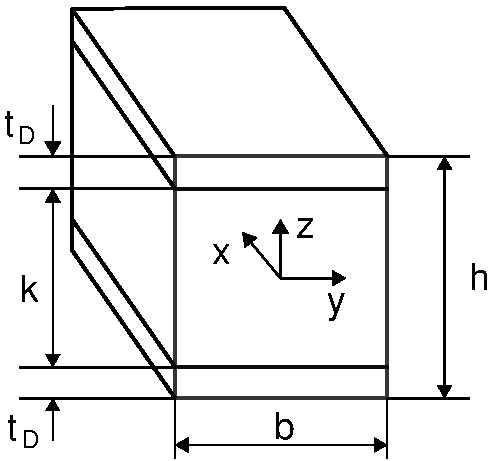
\includegraphics[width=0.3\linewidth]{Bilder/SdT/Aufbau_Dichte_FML}
    \caption[Aufbau eines dreilagigen FML]{Aufbau eines dreilagigen FML mit entsprechender Querschnittszusammensetzung nach~\cite{Wollmann2018}}
    \label{fig:Querschnitt_FML}
\end{figure}

%Metalle
Für Anwendungen in FML wurden anfangs vor allem Aluminiumlegierungen eingesetzt, vorrangig aus den 2000er und 7000er Reihen.
Die daraus entstandenen Verbundwerkstoffe weisen die Vorteile auf, die zur Anwendung führten, wie hohe Schlagenergie, niedrige Risswachstumsgeschwindigkeiten geringe Dichte.
Um das Werkstoffspektrum zu erweitern, wurden Untersuchungen mit anderen Metalllegierungen durchgeführt wie Stählen, Titanlegierungen oder Magnesium.

Neben den weithin verwendeten Aluminiumlegierungen werden Titanbleche für Hochtemperaturanwendungen mit Kohlefasern zu FML verbunden~\cite{Burianek2003,Hu2020}.
Stahlbleche werden vor allem im Hinblick auf Tiefziehoperationen mit FML untersucht, um mit faserversärkten Polymeren die Eigenschaften von klassischen Stahlbauteilen zu verbessern~\cite{Behrens2014,Behrens2017,Blala2021,Hahn2018}.
Magnesium als Metallwerkstoff bietet sich für die Verwendung in FML an, da es als leichtestes Konstruktionsmetall Potenziale im Leichtbau möglich macht und für bestimmte Anwendungen einsetzbar sein kann~\cite{Cortes2005,Alderliesten2008}.
Ein regelmäßig untersuchtes Thema sind die Vorbehandlungsmethoden, um die Oberfläche von Magnesiumblechen oder -bauteilen belastbar an Kunststoffmatrizen anzubinden~\cite{Cicco2019,Cicco2019a}
Intensive Untersuchungen wurden mit Magnesium durchgeführt, um Beschichtungen anzubringen, beispielsweise auf organosilanischer Basis~\cite{Hausbeck2012}.
Die Beschichtungen sind interessant, um die Adsorptionsprozesse von medizinischen Gegenständen aus Magnesium im Körper zu verlangsamen~\cite{Galvin2013,Zucchi2006}.
Die Anbindung der Beschichtung basiert auf den gleichen Prinzipien wie die Anbindung von Kunststoffschichten für mechanisch belastete Werkstoffe wie FML~.

%Kunststoffe/Matrix

Eine wichtige Einteilung von FML kann anhand der verwendeten Kunststoffe oder Matrixwerkstoffe erfolgen.
Für bisherige Anwendungen wurden häufig sogenannte Epoxidharze verwendet, welche aus einem Polymer und einem Härter bestehen.
Beim Mischen entsteht eine Flüssigkeit, die innerhalb einer Zeit aushärtet und einen duroplastischen Kunststoff darstellt~\cite{Dornbusch2015}.
Der Werkstoff ist je nach Zusammensetzung teils spröde und splittert schnell, kann nicht mehr aufgeschmolzen werden und weist hohe mechanische und korrosionsresistente Eigenschaften auf.

Als Laminatwerkstoff kommen die in der klassischen Faserverbundtechnik genutzten Werkstoffe und Verfahren zum Einsatz.
Klassischerweise wurde in den ersten FML wie Glare ein Epoxidharz genutzt, der durch eine chemische Reaktion bei einer erhöhten Temperatur aushärtet.
Der Auftrag erfolgt in einer Serienfertigung durch Prepreg-Material, also vorher imprägnierte Matten von Fasern mit nicht ausgehärtetem Harz, oder andere Verfahren wie Vakuuminfusion.
In den Harzen können Fasern wie Aramid, Glas- oder Kohlefasern zur Verstärkung eingesetzt werden.
Durch die Aushärtung weisen Epoxidharze eine potenziell längere Prozesszeit auf, was aber in aktuellen Entwicklungen weiter verkürzt wird~\cite{Lakho2017}.
Eine in aktuellen Untersuchte Möglichkeit ist der Einsatz von Thermoplasten, also Polymeren wie Polyamid oder Polypropylen~\cite{Flock2012}.
Diese weisen den Vorteil auf, in schmelzflüssigem Zustand gießbar zu sein, und werden in vielen Spritzgußbauteilen angewendet~\cite{Ehrenstein2003}.

Der Vorteil von Thermoplasten ist die geringe Prozesszeit zum Aushärten, da durch ein Abkühlen des Werkstoffes eine Verfestigung eintritt.
Der Vorgang des Aufschmelzens und Abkühlens kann mehrmals wiederholt werden, was mehrstufige Umformoperationen ermöglicht.

Nach Kuhtz et al.~\cite{Kuhtz2019} muss beachtet werden, dass die Haftung der Schichten im Allgemeinen bei der Verwendung von Matrixwerkstoffen auf der Basis von Epoxidharz besser ist als bei thermoplastischen Polymeren.
Ein weiterer Faktor sind die höheren Verarbeitungstemperaturen von Thermoplasten im Vergleich zu Epoxidharzen, die zum Aufschmelzen des Polymers erforderlich sind.
Dadurch können sich erhöhte Eigenspannungen durch unterschiedliche Wärmeausdehnungskoeffizienten ergeben.

Im Gegensatz dazu kommen Polymere ohne Härter aus und weisen thermoplastische Eigenschaften auf.
Ein intensiv genutzter thermoplastischer Werkstoff ist Polyamid, welches sich aus Amidgruppen in verschiedenen Konfigurationen zusammensetzt.
Die Zahl in der Werkstoffbezeichnung bei PA (Beispiel PA6) steht dabei für die Anzahl der Kohlenstoffatome in einer Wiederholungseinheit.
Die Eigenschaften der verschiedenen Polyamide unterscheiden sich kaum~\cite{Flock2012}.
Polyamid erweicht bei höheren Temperaturen und kann somit in eine neue Form gebracht werden.
Zur Erhöhung der Wärmeformbeständigkeit wird PA teilweise mit Glasfasern verstärkt~\cite{Baur2007}.

Behrens et al.~\cite{BerndArno2019} nutzt zusätzlich zum normalen Matrixwerkstoff PA6 mit Kohlefaserverstärkung an den Grenzflächen zu Metallschichten je einen $0,2 \, mm$ dicken Film PA6 ohne Faserverstärkung.
Dieser soll die Haftung verbessern und verhindern, dass sich bei hohen Fügedrücken Fasern direkt an die Metalloberfläche anlegen, ohne dass durch den Matrixwerkstoff eine Haftung entstehen kann.
Dies kann also als Möglichkeit angesehen werden, die Haftfestigkeit ohne zusätzlichen Haftvermittler zu erhöhen.
Ein Nachteil ist der verringerte Faseranteil des Matrixwerkstoffen, so dass dadurch geringere Festigkeiten in Zug- oder Biegebeanspruchungen hervorgerufen werden können.

%Aufbau

Der geometrische Aufbau des Verbundes beeinflusst auch unabhängig von der Materialauswahl die Eigenschaften.
Wie in Untersuchungen gezeigt werden konnte, hat für symmetrische Verbunde die Kerndicke einen großen Einfluss auf die spezifischen mechanischen Eigenschaften.
Wollmann et al.~\cite{Wollmann2018} stellt einem $2\,mm$ dickem Aluminiumblech einen Verbund mit gleicher Dichte gegenüber.
Dieser setzt sich beispielhaft aus zwei Stahlblechen mit $0,25\,mm$ Dicke und einer $1\,mm$ dicken kohlefaserverstärkten Polymerschicht dazwischen zusammen.
In einer weiteren analytischen Betrachtung zeigt sich, dass die mechanischen Eigenschaften stark von der Kerndicke abhängen und mit steigendem Gewichtsanteil der Deckbleche durchweg verschlechtern.
Somit sollte die Blechdicke der Deckbleche in einem dreilagigen Verbund so dünn wie möglich gewählt werden.
Dabei muss die anisotrope Eigenschaftsverteilung der Faserverstärkung besonders beachtet werden.

Diagramm aus Wollmann.18 mit Festigkeit nach Dicke Kern/Bleche


Bild: Einteilung anhand verschiedener Werkstoffe und Aufbauten

%\begin{figure}[H]%[htbp]
%	\centering
%	
\includegraphics[width=0.6\linewidth]{Bilder/SdT/FML_Einordnung}
%	\caption[Einordnung von FML anhand der Metallschicht]{Einordnung von FML anhand verschiedener verwendeter Metallwerkstoffe \cite{Sinmazcelik.2011}
%	\label{fig:Einordnung_FML}
%\end{figure}

Einteilung anhand von: Symmetrie, Anzahl Lagen, Werkstoff Metall, Werkstoff Matrix, Faserverstärkung

\subsection{Haftungsmechanismen}\label{subsec:haftung}


Die sogenannte Haftung ist für die Funktionsweise und Fertigung von FML bedeutend.
Haftung kann als Stärke der Bindung zweier Werkstoffe miteinander definiert werden~\cite{Mann1994}.
Eine andere Definition beschreibt die Haftung $\sigma_H$ als innere Kraft $F_i$ auf die wahre Oberfläche $A_w$ bezogen, was die jeweilige Rauheit der Oberfläche mit einschließt \autoref{eq:Haftung}~\cite{Bischof1993}.

\begin{equation}
    \sigma_H = \frac{F_i}{A_w}
    \label{eq:Haftung}
\end{equation}

Diese innere Kraft kann nicht durch eine einzelne Prüfmethode gemessen werden.
Auch eine Messung der wahren Oberfläche ist nur mit hohem Aufwand und fehlerbehaftet durchführbar~\cite{Brockmann1969}.
Daher wird ein neuer Ausdruck eingeführt, die Verbundfestigkeit $\sigma_v$, die als Quotient der messbaren äußeren Kräfte $F_a$ und der geometrischen Oberfläche $A_g$ definiert ist (siehe \autoref{eq:Verbundfestigkeit}).
Die geometrische Oberfläche entspricht der belasteten Fläche (Breite b und Überlappungslänge l)~\cite{Habenicht2009}.

\begin{equation}
    \sigma_v = \frac{F_a}{A_g}
    \label{eq:Verbundfestigkeit}
\end{equation}

Bei der Belastung des Verbundes kann es zum Bruch an der Verbindung, im Werkstoff oder in einer gemischten Weise kommen.
Dies wird als adhesives oder kohäsives Versagen oder als Mischbruch bezeichnet.
Der Wert $\sigma_v$ muss daher mit den Versagenscharakteristika genannt werden, um eine Aussage über die Haftung zu treffen~\cite{Pan2016}.

Der Begriff der Haftung lässt sich in Adhäsions- und Kohäsionsmechanismen unterteilen.
Im Inneren einer homogenen Werkstoffphase ist die Energieverteilung isotrop, gleichmäßige Kohäsionskräfte bewirken einen Zusammenhalt des Grundwerkstoffs.
An der Oberfläche wirken andere energetische Zustände, die bei der Betrachtung von Grenzflächenvorgängen entscheidend sind.
Die Adhäsion charakterisiert eine Kraft, die in den jeweiligen Oberflächen von zwei Fügepartnern wirkt und dabei vom Abstand der Oberflächen abhängt.
Diese Kraft wird durch die Überlagerung von physikalischen, chemischen und mechanischen Wechselwirkungen an den Grenzflächen der Fügeteile hervorgerufen~\cite{Habenicht2009}~.
Gute Haftungseigenschaften werden auch durch einen geringen Abstand zwischen zwei Fügepartnern, in diesem Fall zwischen Kunststoff und Metall, erreicht.
Molekülabstände zwischen $0,1 - 0,5\, nm$ führen zu hohen Bindungskräften~\cite{Suchentrunk2007}.

Verschiedene Theorien beschreiben die unterschiedlichen Adhäsionsmechanismen.
Dazu zählen die mechanische Adhäsion sowie die spezifische Adhäsion, welche weiter unterteilt werden können.
Einen Überblick darüber verschafft \autoref{fig:Adhasionstheorien}.

\begin{figure}[H]%[htbp]
    \centering
    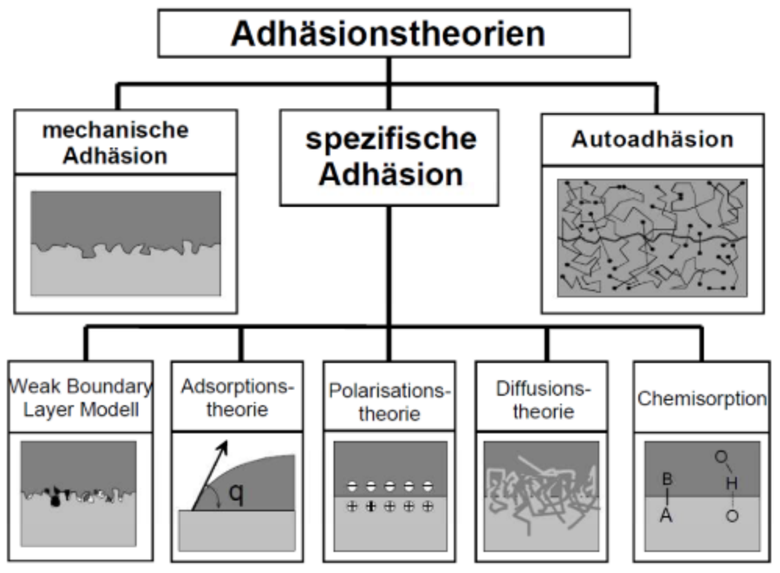
\includegraphics[width=0.6\linewidth]{Bilder/SdT/Adhasionstheorien}
    \caption[Unterteilung der Adhäsionstheorien]{Unterteilung der Adhäsionstheorien nach~\cite{Garbassi1998}}
    \label{fig:Adhasionstheorien}
\end{figure}
%XXX

\subsubsection{Mechanische Adhäsion}

Unter mechanischer Adhäsion wird die geometrische Verankerung eines Stoffes, in diesem Fall des Matrixwerkstoffes, in der Metalloberfläche verstanden.
Durch gezielte Maßnahmen wie dem mechanischen Aufrauen lassen sich zusätzlich zur immer vorhandenen Oberflächenstruktur zusätzliche Kapillaren, Poren und Hinterschneidungen erzeugen.
Wenn der Matrixwerkstoff im flüssigen Zustand in diese Strukturen fließt oder gepresst wird und darin erstarrt, kommt es zu einer formschlüssigen mechanischen Verankerung (auch Druckknopfeffekt genannt), wie in \autoref{fig:Druckknopf} verdeutlicht wird~\cite{Habenicht2009,Mittal1999}.


\begin{figure}[H]%[htbp]
    \centering
    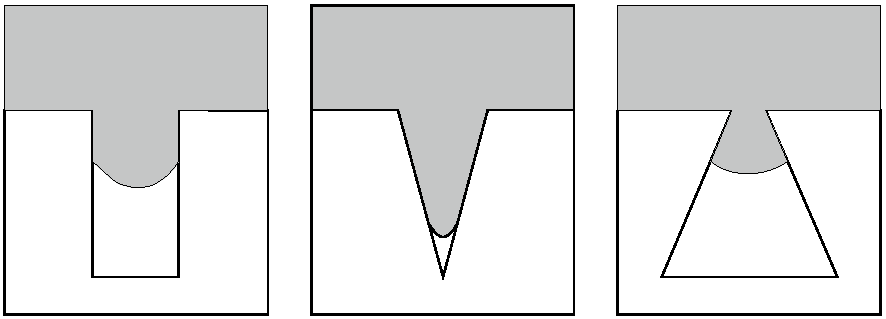
\includegraphics[width=0.6\linewidth]{Bilder/SdT/Druckknopfeffekt}
    \caption[Druckknopfeffekt]{Schematische Darstellung des Druckknopfeffektes~\cite{Mittal1999}}
    \label{fig:Druckknopf}
\end{figure}
%XXX

Die Tiefe des Eindringens in die Struktur ist von den Benetzungseigenschaften des eindringenden Fluids sowie dem Gegendruck des eingeschlossenen Gases abhängig~\cite{Mittal1999}.
Nur ein geringer Anteil der Poren und Oberflächenstrukturen weist die erforderliche Geometrie für eine Verankerung auf.
Jede Oberflächenvergrößerung, auch die nicht für den Druckknopfeffekt geeigneten Poren, führt zu zusätzlichen Beiträgen der einzelnen Haftmechanismen~\cite{Flock2012}.

\subsubsection{Autoadhäsion}\label{subsubsec:autoadhäsion}

Beim Kontakt chemisch identischer Stoffe kommt es zu einer Selbstdiffusion in den Grenzbereichen, bedingt durch die mikrobrownsche Bewegung und abhängig von Zeit, Temperatur und Druck.
Dabei wird eine starke stoffliche Verbindung zwischen den Körpern aufgebaut, allerdings nur bei identischen Werkstoffen.

Für Thermoplaste ist die mikrobrownsche Bewegung von Makromolekülsegmenten von entscheidender Bedeutung für den Effekt der Autoadhäsion.
Dabei sind die Molekülsegmente unterhalb der Glasübergangstemperatur $T_g$ nicht ausreichend beweglich~\cite{Seidler1971}~.
Autoadhäsion findet erst bei Temperaturen über $T_g$ statt.
Einige Kunststoffe wie Polyethylen weisen bei Raumtemperatur kein adhäsives Verhalten auf, während diese makromolekularen Stoffe bei Erwärmung einen adhäsiven Zustand erreichen können~\cite{Seidler1971}

Für Metalle kann das Prinzip der Autoadhäsion nicht angewandt werden, da durch das Metallgitter die Effekte nicht eintreten.
Für FML ist die Autoadhäsion aufgrund der Materialkombination kein zutreffender Haftungsmechanismus~\cite{Flock2012}.

\subsubsection{Spezifische Adhäsion} \label{subsubsec:spez}

Die Theorie der spezifischen Adhäsion setzt sich aus Betrachtungen von chemischen, physikalischen und thermodynamischen Effekten zusammen und gilt im Bereich von $0,2$ bis $1\,nm$~.
Nach~\cite{Garbassi1998} gliedert sich die Theorie in die folgenden Modellvorstellungen.

\paragraph{Weak-Boundary-Layer}

An der Grenzschicht der beiden Fügepartner kann eine sogenannte schwache Grenzschicht (englisch: Weak-Boundary-Layer, WBL) zum Adhäsionsversagen führen.
Diese trennt die beiden Grundwerkstoffe und verhindert eine direkte Anbindung~\cite{Schroeer1994}.
Ursache dafür können Gaseinschlüsse, Verunreinigungen oder auch Oxidationsprodukte auf der Oberfläche sein.
Die WBL kann durch geeignete Vorbehandlungen entfernt werden\cite{Flock2012}.

\paragraph{Polarisationstheorie}

Der Polarisationstheorie zufolge führt die Existenz polarer funktioneller Gruppen in den beiden Grundwerkstoffen bei geringem Abstand (<$5\cdot10^[(-10)] \, m$) zu einer Kraftwirkung, die als Adhäsion bezeichnet werden kann.
Grund für die Krafteinwirkung sind Wasserstoffbrücken und Dipolwechselwirkungen~\cite{Weiss2002}.
Die Bindungskräfte sind abhängig vom Dipolmoment der Atome bzw.\ Moleküle und lassen sich durch den Einbau von sauerstoffhaltigen funktionellen Gruppen verbessern~\cite{Garbassi1998}.
Die in unpolaren Werkstoffen auftretenden Bindungskräfte können mit dieser Theorie nicht erklärt werden~\cite{Habenicht2009}.

\paragraph{Diffusionstheorie}

Anlehnend an die Autoadhäsionstheorie erklärt die Diffusionstheorie auftretende Bindungskräfte mit einer Selbstdiffusion von Molekülsegmenten innerhalb der Grenzschicht der Fügeteile~\cite{Gromov1963}.
Auch diese Diffusionsbewegungen können mit der mikrobrownschen Molekularbewegung begründet werden.
Neben der chemischen Verträglichkeit der Fügeteile muss die Molekularmasse und -struktur sowie der Kristallinitäts- und Vernetzungsgrad der Polymere beachtet werden~\cite{Habenicht2009}.
Für FML ist die Diffusionstheorie nur bei Verwendung eines Haftvermittlers relevant,  da sich dieser an das Metall anbindet und eine Diffusion zwischen Haftvermittler und Polymer stattfindet~\cite{Suchentrunk2007}.
Andere Untersuchungen konnten einen Diffusionseffekt an der Grenzschicht von Metall und Polymer und eine Bewegung von Metallatomen in die Kunststoffschicht beobachten~\cite{Faupel2003}.

\paragraph{Chemiesorption}

Chemiesorption (Kurzform von chemischer Adhäsion) bedeutet die Bindung von Molekülen durch eine kovalente Bindung an der Oberfläche des Substrats.
Diese Bindungen lassen sich nicht einfach Nachweisen, allerdings wurden exotherme Reaktionen und zwischen Kupfer und Polymeren beobachtet, die auf eine chemische Bindung an der Grenzfläche zu Kupfer schließen lassen~\cite{Schroeer1994}.
Im Zusammenhang mit FML wird der Effekt der Chemiesorption vorrangig im Zusammenhang mit der Verwendung von Haftvermittler betrachtet.
Dieser ist auf die Fügepartner abgestimmt und sorgt für eine chemische Anbindung der Werkstoffe.
Haftvermittler basieren teilweise auf siliziumorganischen Verbindungen und werden auf die Oberfläche des Metalls aufgetragen~\cite{Zucchi2006}.
Bei richtiger Abstimmung wird die Festigkeit der Klebung und die Beständigkeit von Klebung und Oberfläche gegen feuchte Atmosphäre verbessert~\cite{Habenicht2009}.

\subsubsection{Oberflächenenergie}\label{subsubsec:eoberfläche}

Die Oberflächenenergie wird als Arbeit definiert, die aufgewendet werden muss um eine Oberfläche um eine Flächeneinheit zu vergrößern~\cite{Flock2012}.
Benetzung bedeutet die Verteilung einer Flüssigkeit auf einer festen Oberfläche.
Ändert sich der Phasenzustand der Flüssigkeit und erstarrt diese an der Oberfläche, wird diese Benetzung mit Adhesion gleichgesetzt~\cite{Habenicht2009}.
Je höher die Oberflächenenergie des Feststoffes im Vergleich zur Oberflächenenergie der Flüssigkeit ist, desto besser ist die Benetzungsfähigkeit der flüssigen Phase~\cite{Flock2012}.
Durch die Kenntnis der Oberflächenenergien der Fügepartner kann also eine quantitative Bewertung der der Adhäsionsenergien durchgeführt werden~\cite{Nikolova2005}.
Die Einschätzung von Oberflächenenergien kann anhand der Tropfenmethode durchgeführt werden, bei der ein Wassertropfen an der zu untersuchenden Oberfläche hängt und anhand der Tropfenform bzw.\ Kontaktwinkel die Oberflächenspannung errechnet werden kann~\cite{Flock2012}.

Weitere Infos zur Tropfenmethode

Die Oberflächenenergie beeinflusst die Benetzungsfähigkeit der Oberfläche mit einer Flüssigkeit und kann auf verschiedene Arten modifiziert werden.
Ähnlich wie die mechanische Adhesion kann die Oberflächenenergie durch das Einbringen einer zusätzlichen Rauheit in die Oberfläche erhöht werden.
Auch chemische oder plasmaelektrische Verfahren werden dazu angewendet XXXQuellen.

\subsubsection{Grenzschichtmodelle}\label{subsubsec:modelle}

Bei der flächigen Verbindung von Metall und Kunststoff bildet sich eine Grenzschicht aus, welche die auftretende Haftung beeinflusst.
Nach~\cite{Haefer1987} gibt es fünf verschiedene Möglichkeiten zur Ausbildung dieser Grenzschicht, welche sich in der jeweils gebildeten Mikrostruktur unterscheiden.
Für den Fall von FML können die frei folgenden Modelle angewendet werden~\cite{Flock2012}.

\paragraph{Monoschicht - Monoschicht}

Es wird ein scharfer Übergang zwischen Metall und Polymer ausgebildet, welcher innerhalb weniger Atomlagen stattfindet.
Dies tritt auf, wenn Verunreinigungen an der Oberfläche vorliegen oder die Stoffe nicht ineinander löslich sind.
Chemische Bindungen oder Diffusionsprozesse treten selten oder gar nicht auf~\cite{Mann1994,Haefer1987}.

\paragraph{Mechanische Verankerung}

Voraussetzung für mechanische Verankerung sind raue, unebene oder poröse Oberflächen.
Das Polymer erstarrt in den Unebenheiten und verankert sich im Metall, wenn die Oberfläche benetzbar und das flüssige Polymer beweglich ist~\cite{Haefer1987}.
Die Haftung beruht also ausschließlich auf dem Formschluss der beiden Fügeteile~\cite{Flock2012}.

\paragraph{Chemische Bindung}

Bei der chemischen Bindung bildet sich die Grenzschicht durch einen konstanten chemischen Aufbau über mehrere Atomlagen hinweg aus.
Die Haftung ist das Resultat chemischer Reaktionen zwischen Metall und Polymer~\cite{Haefer987}.
Voraussetzung ist die Reaktionsfähigkeit der Oberflächen, die durch Oxidation, Verschmutzung oder Verunreinigung herabgesetzt werden kann.

\paragraph{Reale Grenzschicht}

Die drei beschriebenen Grenzschichten treten in der Realität nicht getrennt voneinander auf, so dass sich aus der Wechselwirkung eine reale Grenzschicht ergibt.
Diese reale Grenzschicht bildet sich abhängig von der Materialkombination, vom Zustand der Ausgangsmaterialien sowie von den Verarbeitungsbedingungen aus~\cite{Flock2012}.

\subsubsection{Beeinflussung der Haftung zwischen Metall und Kunststoff}\label{subsubsec:beeinflussung}

Eine entscheidendes Kriterium für die Verwendung von FML ist es, einen haltbaren und festen Verbund zwischen den einzelnen Lagen sicherzustellen.
Wie in \autoref{eq:Haftung} dargelegt, sind nicht alle Mechanismen auf die Verbindung von Metall zu Kunststoffen übertragbar.
Darum gilt es, Verfahren anzuwenden, die die Haftung in FML erhöhen.
Dazu gibt es verschiedene Ansätze wie das mechanische Aufrauen der Oberfläche, eine chemische Behandlung mit Beizen, Beschichtungen, das Aufbringen von Haftvermittlern auf die Metalloberfläche und plasmaelektrische Verfahren.
Diese Möglichkeiten sollen hier vorgestellt werden.

Zhou et al.~\cite{Zhou2021} stellt eine Möglichkeit vor, mit der FML auf Magnesiumbasis mithilfe einer Zwischenschicht aus einer eutektischen Mg-Zn-Al-Legierung haltbar verbunden werden.
Dazu wurden die Bleche mit Sandstrahlen und Beizen vorbehandelt und mit der Zwischenschicht und einer Epoxidharzmatrix im Heißpressverfahren unter Ultraschalleinwirkung gefügt.
Zusätzlich wurden die Kohlefasern mit einer Ni-Schicht beschichtet, um eine bessere Verteilung des Epoxidharzes zu erreichen.
Es konnte gezeigt werden, dass sich ein circa $350 \, \mu m$ breiter Übergangsbereich ausbildet, der Anteile an Magnesium-, Aluminium-, Zink- und Kohlenstoffatomen aufweist.
Dieser Bereich wird sowohl durch die Applikation der Zwischenschicht als auch durch Diffusion aufgebaut.
Eine deutlich höhere interlaminare Festigkeit ist zu beobachten, da über die Zwischenschicht die Fasern besser an das Magnesiumblech angebunden werden.
Dies führt zu erhöhten Biege- und Zugfestigkeiten des Verbundes.
Der Verbund versagt ungefähr zeitgleich adhäsiv und kohäsiv in der Matrix, so dass eine optimale Ausnutzung der Werkstoffe erreicht wurde.

Ein andere Möglichkeit der Oberflächenvorbehandlung zeigt Wu et al.~\cite{Wu2016}.
Gegenüber klassischen mechanischen Methoden oder Lasereinsatz hat eine Vorbehandlung durch eine Art Funkenerosion verbunden mit einem Beizprozess ($CrO_3$-Lösung) Vorteile hinsichtlich der geometrischen Flexibilität und der effizienten Anwendbarkeit bei größeren Bauteilen und Stückzahlen.
Auch hat dieser \glqq microarc\grqq genannte Funkenerosionsprozess große Vorteile hinsichtlich des Korrosionsschutzes und Hydrophobie und führt zu selbstreinigenden Oberflächen~\cite{Lu2015}.
Mit den genannten Methoden konnte eine Oberfläche mit sehr hoher Rauheit und Mikro- und Nanooberflächenstrukturen erzeugt werden, die hervorragende wasserabweisende und damit verbindungsfähige Eigenschaften aufweist.

Eine Möglichkeit zur Verbesserung der Haftung stellt Staiger et al.~\cite{Staiger2014} vor.
In der Untersuchung werden unter anderem die Metalloberflächen mit Sandstrahlen und Plasmabehandlung bearbeitet.
Eine bisher wenig betrachtete Möglichkeit ist die Vorbehandlung des Matrixwerkstoffes, in diesem Fall Polypropylen (PP), mit einer Plasmafunktionalisierung.
Dabei werden durch kurze Plasmaentladungen an der Oberfläche funktionale Gruppen angebunden und die adhäsiven Eigenschaften des Matrixwerkstoffes deutlich verbessert.

Flock~\cite{Flock2012} verglich die Haftfestigkeiten von Stahl und Aluminium mit verschiedenen thermoplastischen Polymeren, unter anderen PA66 mit und ohne Glasfaserverstärkung.
Dabei wurde für PA66 die höchste Scherzugfestigkeit nachgewiesen, ohne Faserverstärkung wurde eine Mischform zwischen kohäsivem und adhäsivem Versagen beobachtet.
Mit eingebrachten Glasfasern versagte der Probenverbund rein adhäsiv.
Von den untersuchten Oberflächenvorbehandlungen konnte die laserstrukturierte Oberfläche mit eigens eingebrachten Hinterschnitten die bei weitem höchste Zugscherfestigkeit verzeichnen.
Von den anderen untersuchten Methoden konnte das Sandstrahlen die vergleichsweise höchsten Zugscherfestigkeiten erreichen.
Die Plasmaaktivierung der Oberfläche hat einen geringen Einfluss auf die Haftung, diese wird durch den Einsatz aber reproduzierbarer, da die Streuung der Ergebnisse reduziert wird.
Die Fügetemperatur wird zwischen \SI{230}{\degreeCelsius} und \SI{270}{\degreeCelsius} variiert.
Je höher die Fügetemperatur ist, desto besser werden die Haftungseigenschaften, allerdings sinkt für \SI{280}{\degreeCelsius} die Scherzugfestigkeit.
Das kann mit dem seitlichen Austreiben des verflüssigten Kunststoffes aus dem Fügebereich erklärt werden.
Dadurch liegen teils Glasfasern direkt am Metall an, ohne dass eine Haftung durch den Matrixwerkstoff hergestellt wird.
Somit ist eine zu hohe Fügetemperatur nachteilig und als Optimum wird \SI{270}{\degreeCelsius} festgestellt.

Bild Laserstrukturiert von Flock

Eine Möglichkeit der Beeinflussung der Oberflächenenergie stellt Gupta et al.~\cite{Gupta2012} vor.
In der Untersuchung wird AZ31 mit Schwefelsäure geätzt und danach mit einer Wasserstoffperoxid-Lösung behandelt.
Dabei konnte die Veränderung des Kontaktwinkels eines Wassertropfens von \ang{140} auf \ang{152} gesteigert werden, was auf eine Erhöhung der Oberflächenenergie hindeutet.
Die bei der Vorbehandlung entstehenden Oberflächenstrukturen sind platten- oder nadelförmig aufgebaut und bestehen hauptsächlich aus Magnesium-Wasserstoffverbindungen.
Die Untersuchung der Korrosionsbeständigkeit zeigt schlechtere Ergebnisse für geätzte im Vergleich zu geschliffenen Proben.
Dies kann auf die erhöhte Oberflächenrauheit zurückgeführt werden, da Oxidationsprozesse aufgrund der größeren Oberfläche schneller ablaufen.

Eine speziell für Magnesiumlegierungen vorgeschlagene Möglichkeit der Klebevorbereitung ist eine kombinierte mechanische und chemische Oberflächenbehandlung.
Dazu schlägt~\cite{Bauer1991} einen vorgeschalteten Strahl- und Schleifschritt vor, um die auf der Oberfläche haftenden Oxide und andere Verunreinigungen mechanisch zu entfernen.
Danach schließt sich ein Beizprozess mit einer Lösung aus Salzsäure ($HCl$), Salpetersäure ($HNO_3$) und Dichromsäure ($H_{2}Cr_{2}O_{7}$) an.
Der Beizvorgang soll bei Raumtemperatur und für eine Minute durchgeführt werden.
Abschließend soll die Probe mit Wasser abgespült werden.
Diese Empfehlung wird allgemeingültig für alle Magnesiumlegierungen vorgeschlagen, obwohl eine Anpassung an die jeweilige Zusammensetzung erforderlich sein kann.
Die Kombination aus mechanischen und chemischen Verfahren bietet den Vorteil, auch starke Oberflächenverunreinigungen und Oxide zuverlässig zu entfernen.
Durch eine Variation der mechanischen Vorbehandlung kann eine erwünschte Rauigkeit eingestellt werden.

\subsection{Herstellung}\label{subsec:herstellung}

Kategorisieren nach Zusammensetzung.
Laminierte Verbunde
Trocken zusammengelegt
Eingegossen

Es gibt mehrere Möglichkeiten, Verbunde zwischen Metall und Kunststoff herzustellen.
Eine Möglichkeit ist das sogenannte Hybridspritzgießen~\cite{GeigerManfred2003}.
Das Verfahren kann genutzt werden, um Blechbauteile durch Hinterspritzungen mit Polymeren zu versteifen und Funktionen wie Einschraubteile zu integrieren.
Dabei werden die Prozessschritte Blechumformen und Verbundherstellung bisher getrennt, auch wenn es Ansätze gibt um die Verfahrensschritte zu kombinieren~\cite{Wiedemann2017}.

Ein wichtiger Faktor sind die Verarbeitungstemperaturen des Verbundes.
Für thermoplastische Matrixwerkstoffe müssen höhere Temperaturen angewendet werden, was auch zu höheren Eigenspannungen im Verbund führt und somit die Lebensdauer verringert~\cite{Alderliesten2008}.

Die grundsätzliche Herstellung von FML gestaltet sich unabhängig der Zusammensetzung des Verbundes immer ähnlich.
Im ersten Schritt werden die einzelnen Werkstoffe vorbereitet, beispielsweise Oberflächen aufgeraut oder entfettet.
Danach werden die Lagen in einem Werkzeug oder ähnlichem zusammengeführt, so dass der Aufbau lose gepackt (englisch \glqq stacking\grqq).
Im dritten Schritt wird eine Temperaturerhöhung durchgeführt sowie eine flächige Druckbeaufschlagung.
Die erforderliche Temperatur richtet sich nach dem verwendeten Matrixwerkstoff.

\subsubsection{Vorbereitung}

Wie in \autoref{subsec:haftung} beschrieben, gibt es verschiedene Ansätze und Technologien für eine Oberflächenvorbehandlung.
An dieser Stelle sollen Referenzen genannt werden, um die Implementierung anhand der Ergebnisse der Untersuchungen auszurichten.

Um die Haftung zwischen den Lagen eines Verbundwerkstoffes zu optimieren, können mechanische, chemische, elektrische oder Beschichtungsprozesse angewendet werden.
Diese sorgen für die Anwendung der in \autoref{subsec:haftung} beschriebenen Effekte.
In den meisten Fällen werden chemische Bindungen sowie ein mechanisches Verklammern der Oberflächen durch erhöhte Oberflächenrauheit angestrebt.

Eine Oberflächenrauheit kann durch Sand- oder Partikelstrahlen, Schleifen, Prägen, Laserstrukturieren, oder andere Prozesse eingebracht werden.
XXXY

Kuhtz et al.~\cite{Kuhtz2019} stellt eine Möglichkeit der mechanischen Oberflächenvorbehandlung mit Prägewerkzeugen vor.
In diese können mit unterschiedlichen Methoden Strukturen eingebracht werden, welche bis zu $300\, \mu m$ hohe regelmäßige oder unregelmäßige Rauheiten in Bleche einbringen können.
Diese Oberflächenstrukturen sorgen für eine mechanische Bindung, welche durch chemische Vorbehandlungen und damit verbundene molekulare Bindung in der Grenzschicht verbessert werden können (siehe auch \autoref{fig:Adhasionstheorien}).
Die Prägewerkzeuge wurden mit eine Flächenpressung von $125\, MPa$ auf die Werkstücke gedrückt und somit die Oberflächenstrukturen in Bleche der Magnesiumlegierung AZ31 und Aluminiumlegierung AL 5754 eingebracht.
Höhere Pressungen führten nicht gleichmäßig zu einer Erhöhung der Rauheit der Blechoberfläche.
Es konnte keine komplette Übertragung der Rauheit festgestellt werden.

Flock~\cite{Flock2012} stellt fest, dass eine laserstrukturierte Oberfläche zu hervorragenden Haftungseigenschaften führt, allerdings eine aufwendiges Verfahren darstellt.
Eine Verwendung bei größeren Flächen schließt der Autor aus und begründet so, dass Verfahren nicht für eine Serienfertigung einzusetzen.
Als im Verhältnis zum Aufwand gutes Verfahren wird das Sandstrahlen der Oberfläche vorgeschlagen, da so gute Rauigkeiten mit etablierter Technik erreicht werden können.
Auch eine Plasmabehandlung der Oberfläche verbessert die Haftung für PA66 deutlich, stellt allerdings auch ein aufwendiges Verfahren dar.

Pan et al.~\cite{Pan2016} stellte einen Verbund aus Magnesiumblechen der Legierung AZ31 und einer Epoxidharzmatrix mit unidirektionalen Kohlenfaserverstärkungen her.
Dazu wurde das Blech mit Aluminiumoxidpartikeln bestrahlt, um die Oberfläche aufzurauen.
Vor dem Fügeprozess wurde das Blech mit Aceton gereinigt.
Durch die Erhöhung der Oberflächenrauheit konnte ein höherer Effekt der mechanischen Verankerung erreicht werden.
Allerdings schließt die Untersuchung mit dem Hinweis auf erforderliche weitere Vorbehandlungen wie Beizprozesse oder dem Einsatz von Haftvermittlern, da die in der Studie angewendete Strategie nur zu einem Bruchteil der möglichen und erforderlichen Festigkeit geführt hat.

Im LEIKA Projekt~\cite{Wiedemann2017} wurden Verbunde aus Magnesiumblechen mit Matrixwerkstoffen und einer Faserverstärkung hergestellt und Strategien zur Verbesserung der Haftung untersucht.
Als Matrixwerkstoff wurde der Thermoplast Polyamid 6 verwendet.
Faserverstärkungen aus Kohlefaser und Glasfasern wurden untersucht.
Die Oberfläche des Magnesiumblechs aus der Legierung AZ31B wurde mit sauren oder basischen Lösungen behandelt, um die nichtmetallischen Bestandteile des Oberflächenaufbaus abzulösen, die beim stark oxidierenden Magnesium auf der Oberfläche gebildet werden.
Bei diesem Prozess wird die native Metalloberfläche passiviert und mit stark polaren Gruppen versehen.
An diese Gruppen bindet sich der organische Polymeranteil des Haftvermittlers und sorgt für eine Verdichtung der Grenzschicht, so dass eine festere Verbindung zwischen Polymermatrix und Metalloberfläche entsteht.
Außerdem vermindert der vorher aufgetragene Haftvermittler die erneute Korrosion der Metalloberfläche.

Kazemi et al.~\cite{Kazemi2020} untersuchte die Einflüsse von Oberflächenvorbehandlungen auf die Eigenschaften eines Verbundes von Titan und kohlefaserverstärktem Epoxidharz.
Unter anderem wurden Sandstrahl-, elektrochemische, elektrolytische, chemische Beiz- und Oxidationsprozesse untersucht.
Mikrolichtbogenoxidation stellte sich dabei als sehr effektive, aber auch aufwendige Methode der Oberflächenvorbehandlung heraus.

Hausbeck~\cite{Hausbeck2012} untersuchte die Beschichtung von medizinischen Stents aus der biodegradablen Magnesiumlegierung WE43 mit sogenannten funktionellen Organosilanen, um die Korrosionsprozesse und den Materialabbau zu verlangsamen.
Die Organosilane binden sich mit kovalenten Bindungen an das Metall an, was durch Oxide und andere Verunreinigungen an der Oberfläche behindert wird.
Eine vorgestellte Möglichkeit ist das Säubern der Proben mit Salpetersäure.
Dazu wird eine Lösung mit $80\, \frac{g}{l}$ Salpetersäure hergestellt (beispielsweise $82,23 ml HNO_3$ auf einen Liter mit Reinstwasser aufgefüllt)~.
Die so hergestellte Lösung wird schnell gerührt und die Probe für circa 2 Sekunden eingetaucht.
Nach dieser vergleichsweise geringen Einwirkzeit sind die Verunreinigungen abgelöst.
Als weitere Vorbereitung zur Anbindung von Silanen schlägt~\cite{Hausbeck2012} einen Tauchschritt mit gesättigter isopropanolischer Natronlauge unter Ultraschalleinwirkung vor.
Diese Natronvorbehandlung wirkt sich sehr günstig auf die Anbindungsfähigkeit der Silangruppen aus, da so an der Magnesiumoberfläche Hydroxidgruppen gebildet werden~\cite{Hausbeck2012,Goubaidoulline2004}, hat aber keinen Einfluss auf die Reinheit der Oberfläche.

Ein Möglichkeit der Oberflächenvorbehandlung stellt das sogenannte microarc oxidation-Verfahren dar, welches durch Stromeinwirkung eine keramische Schicht an der Oberfläche des Substrates entstehen lässt.
verschiedene Elektrolyte (Lösungen) möglich, meist wässrige Lösungen mit Si- oder P Anteil.
Cai et al.~\cite{Cai2006} untersucht die Auswirkung auf AZ91.
je nach Elektrolyt schichtdicke von ca. $20 \, \mu m$ eingestellt, und andere Schichtzusammensetzung.
Auch Spannung beeinflusst Schichtzusammensetzung, Porosität und Morphologie.
deutlich verbesserte Korrosionseigenschaften.

\subsubsection{Fügeprozesse}

Der Fügeprozess schließt sich an einen Stacking-Vorgang an, also das Schichten der unterschiedlichen Lagen zu einem losen Verbund.

Mousa et al.~\cite{Mousa2017} untersuchte die Herstellung eines dreilagigen Verbundes durch direktes Warmrollfügen.
Dabei werden die einzelnen Schichten, in diesem Fall zwei Bleche und eine Polymerschicht ohne zusätzliche Faserverstärkung, in einem kontinuierlichen Prozess erwärmt und zwischen zwei Walzen zusammengepresst.
Vor dem Fügevorgang wurden die für die Versuche genutzten Al 1100 Bleche mit Ethanol gereinigt und mit einem Schleifpapier (Körnung 50) abgeschliffen, so dass eine Rauheit von $5,6\, \mu m$ erreicht werden konnte.
Nach der Oberflächenvorbehandlung und der Erwärmung der Blechoberflächen wurden die drei Lagen gestapelt und durch Walzen mit $65\, mm$ Durchmesser in der Dicke reduziert (bei 30 rpm).
Eine Dickenreduktion von $60 \%$ stellte sich dabei als optimal heraus bezüglich einer hohen zu erreichenden Schälfestigkeit.
Der Grund dafür ist die verbesserte Haftung durch höhere Anpressdrücke und den damit verbundenen interlock des Polymers an der Metalloberfläche.
Eine Dickenreduktion um $75\%$ zeigte eine geringere Schälfestigkeit, da die hohen Anpressdrücke zum seitlichen Austreten des Kunststoffes aus dem Verbund führten.
Dabei kommen Fasern in direkten Kontakt mit einer Metalllage, was keine Haftung erzeugt.

Ein klassischer Ansatz für die Fertigung von faserversärkten Kunststoffbauteilen ist die Anwendung von Vakuumtechnik, um einen erforderlichen Druck aufzubauen, und noch gebundene Gase aus dem Matrixwerkstoff zu ziehen.
Das Verfahren funktioniert über eine Folien, welche das Bauteil abdichtet, und einen Schlauch, über eine Vakuumpumpe eine Druckminderung im abgedichteten Bereich erreicht.
Durch den Unterschied zum Umgebungsdruck wird der Matrixwerkstoff verdichtet und Lufteinschlüsse werden entfernt.
Die Technik wird häufig bei Epoxidharzbauteilen verwendet~\cite{Bellini2020}.
Der Aufbau mit evakuiertem Vakuumsack wird erhitzt, was zur Aushärtung führt.
Thermoplastische Matrixwerkstoffe können meist ohne Vakuumeinsatz verarbeitet werden, da durch ein separates Extrudierverfahren feste Bauteile ohne weitere Gaseinschlüsse hergestellt werden können.

Bei Epoxidharzen muss die Aushärtetemperatur erreicht und für eine bestimmte Zeit gehalten werden, bei Polymerkunststoffen wie PA wird die Glasübergangstemperatur überschritten, so dass der Kunststoff mindestens teilweise verflüssigt.
Durch den applizierten Druck, beispielsweise mit einem Stempel oder durch Vakuumeinfluss, wird der Matrixwerkstoff in die Vertiefungen der Metalloberfläche gedrückt, so dass die Rauheiten weitgehend ausgefüllt werden.
Epoxidharze härten bei der Temperatur über längere Zeiträume aus, während für Polymere die Temperatur wieder gesenkt, der Druck aber aufrechterhalten wird.
Somit ergibt sich eine starre Matrix, welche die Fasern miteinander und mit den Metallblechen verbindet~\cite{Sinmazcelik2011}.

Da die Aushärtezeiten von Epoxidharzen sehr lang sein können, wurden die Bauteile meist einzeln gefertigt und häufig per Hand vorbereitet.
Dieses Verfahren bedingt den hohen Preis der Bauteile und führt zu einem geringen Automatisierungsgrad.
Thermoplaste müssen nur erwärmt und abgekühlt werden, was auch innerhalb einer kurzen Zeit erfolgen kann.
Das Potenzial für eine Serienfertigung ist bei Verwendung von thermoplastischen Kunststoffen daher höher und wird intensiv untersucht.

Eine Produktionsmöglichkeit ist das sogenannte Roll Forming, also das fügen von FML in einem kontinuierlichen, dem Plattieren ähnlichen Walzprozess.
Dabei können auch Profile aus mehreren Lagen hergestellt werden, sowohl mit Prepreg-Verfahren (Epoxidharzmatrix, welche im Anschluss ausgehärtet wird) als auch mit thermoplastischer Matrix~\cite{Long.2007}.
Das Verfahren bietet Vorteile hinsichtlich der geringeren Rückfederung und Eigenspannung.
Ein Auspressen des Matrixwerkstoffes kann durch ungleiche Druckverteilung während der Umformung auftreten~\cite{Sinke2007}.

Mousa~\cite{Mousa2015} stellt fest, dass eine erhöhte Rauheit zwar die Oberfläche vergrößert, allerdings auch eine Benetzung durch ein Polymer durch zu kleine Oberflächenstrukturen behindert werden kann.
Zusätzlich bilden eingebrachte Rauheiten immer Spannungskonzentrationsstellen und können somit Anrisse begünstigen.

Nach Kuhtz et al.~\cite{Kuhtz2019} muss beachtet werden, dass die Haftung der Schichten im Allgemeinen bei der Verwendung von harzbasierten Matrixwerkstoffen besser ist als bei thermoplastischen Polymeren.
Ein weiterer Faktor sind die höheren Verarbeitungstemperaturen von Thermoplasten im Vergleich zu Epoxidharzen, die zum Aufschmelzen des Polymers erforderlich sind.
Dadurch können sich erhöhte Eigenspannungen durch unterschiedliche Wärmeausdehnungskoeffizienten ergeben.
In der vorliegenden Untersuchung werden die Bleche mit Prägewerkzeugen aufgeraut.
Die Fertigung der Proben wurde mit einem auf Polyolefinen basierten Haftvermittler Cox 391 von Nolax durchgeführt.
Die geprägten Metallbleche wurden mit dem Laminat-Tape (PA6 Matrix mit Kohlefaserverstärkung) gestapelt und der Verbund auf \SI{250}{\degreeCelsius} erhitzt.

Für die Herstellung von geringen Stückzahlen beispielsweise in der Luftfahrt ist daher eine Verwendung von Epoxidharz denkbar, allerdings ist die Anwendung von thermoplastischen Kunststoffen aufgrund der geringeren Verarbeitungszeit deutlich besser für eine Massenfertigung geeignet.
Thermoplaste können mehrmals aufgeschmolzen werden, was eine Umformung in mehreren Schritten ermöglicht~\cite{Reyes2000, Wollmann2018}.


Durch die Verwendung von zusätzlichen Kunststofflagen ohne Faserverstärkung an den Grenzflächen zur jeweiligen Metalllage kann die Haftung deutlich verbessert werden, da so ein direkter Kontakt zwischen Fasern und Metall verhindert wird.
Zudem kann eine ideale Benetzung stattfinden~\cite{Marissen1988}.

Pärnänen et al.~\cite{Paernaenen2012} untersuchte die Möglichkeit der Herstellung von FML mit der Magnesiumlegierung AZ31B-H24 und verglich die Versagenseigenschaften des Verbundes mit bestehenden Glare Werkstoffen (Glare 5-3/2-0,4 und Glare 5-3/2-0,5).
Dabei wurde als Blechwerkstoff ein 0,5 mm dickes Magnesiumblech der genannten Legierung genutzt, welches mit einem Salpertersäurebad und leichtem Sandstrahlen vorbehandelt wurde.

Alderliesten~\cite{Alderliesten2009} stellt fest, dass durch die Wärmeeinwirkung während der Herstellung von Verbundwerkstoffen Eigenspannungen entstehen, da Metalle, Matrixwerkstoffe und Fasern unterschiedliche Kontraktionen beim Abkühlen erfahren.
Diese Spannungen wirken sich negativ auf das gewünschte Eigenschaftsprofil aus und können zu frühzeitigem unkontrollierten Risswachstum, ungünstigem Versagensverhalten, Verzug sowie adhäsivem Versagen führen.
Um die Nachteile der entstehenden Spannungen umzukehren, können komplett gefügte Bauteile in einer Streckziehoperation bis zur plastischen Deformation gezogen werden.
Dazu schlägt~\cite{Delft.1} das Einspannen des Bauteils von beiden Seiten mit Klemmbacken vor, ohne die Oberfläche zu beschädigen.
Eine andere Möglichkeit ist die Verwendung von Walzen, um eine minimale Dickenreduktion des Verbundes und damit eine leichte Überlagerung der Spannungen zu erzielen~\cite{Vogelesang1989}.

Staiger et al.~\cite{Staiger2014} stellt eine Möglichkeit vor, das Fügen von Thermoplast zu Faserverstärkung im gleichen Schritt erfolgen zu lassen wie den Fügeprozess von Metall zum Matrixwerkstoff.
Dazu können Fasern aus thermoplastischen Kunststoffen mit den Verstärkungsfasern verwebt, aber nicht erhitzt werden.
Diese Gewebematten sollen dann mit den Blechen gestapelt werden.
In diesem Zustand kann durch erhitzen das Gewebe teilweise aufgeschmolzen und eine Haftung eingestellt werden.
Der Vorteil dieses Verfahrens ist, dass auch die Fasern vorher beschichtet werden können, um eine verbesserte Haftung zwischen Matrixwerkstoff und Faserverstärkung einzustellen.


Bild von unterschiedlichen Schermodi


Die Fertigungsversuche in~\cite{Wiedemann2017} wurden in drei Schritten durchgeführt.
Im ersten Schritt wurden Faseranteile, Polymermatrixfolien und die Metallbleche mit aufgetragenem Haftvermittler gestapelt.
Durch Erwärmung und Druckbeaufschlagung in einer Presse wurden die Polymeranteile aufgeschmolzen und somit die Faseranteile imprägniert.
Eine formschlüssige Verbindung von Metall zu Polymer sowie Polymer zu Faseranteil wurde durch das Abkühlen des Kunststoffes im dritten Verfahrensschritt hergestellt.
In diesem wurden die Verbunde auf die Zieldicke konsolidiert, aus der Presse entnommen und nachbearbeitet.
Für die Erwärmungszone wurde eine Werkzeugtemperatur von $280\, ^\circ \text{C}$ gewählt bei einer Heizdauer von $130 s$.
Die Werkzeuge für die Abkühlstufe wurden mit $80\, ^\circ\text{C} C$ temperiert und für jeweils $30\, s$ eingesetzt\cite{Wiedemann2017}.

Bild von LEIKA über Stufen der Fertigung

Carrado et al.~\cite{Carrado2010} stellt einen Fügeprozess mithilfe einer Rollenvorrichtung vor.
Dieser Vorgang wird als Press-Joining-Rolling bezeichnet, übersetzt Pressfügerollen.
Dabei werden die Metallkomponenten, in diesem Fall zwei Stahlbleche, erst gereinigt und mit einem Epoxidharz als Kleber beschichtet.
Nach einer Erwärmung auf \SI{254}{\degreeCelsius} wird das untere Blech in der Rollvorrichtung zwischen zwei Walzen mit einer thermoplastischen Folie gefügt.
Nach der Erwärmung des oberen Bleches wird ein dreilagiger symmetrische Sandwichwerkstoff in der Rollanlage zweistufig hergestellt.

\subsubsection{Weiterverarbeitung}

Behrens et al.~\cite{Behrens2014} zeigt eine Möglichkeit auf, aus vorbehandelten Werkstoffen in einem Schritt einen dreidimensionalen Verbund herzustellen.
Dazu wird mit erhöhten Temperaturen gearbeitet, um den thermoplastischen Matrixwerkstoff formbar zu machen.
Das Konzept des Tiefziehens thermoplastischer Werkstoffe wird als Thermoforming bezeichnet und unter anderem von Engelmann et al.~\cite{Engelmann2012} beschrieben.
Die Tiefziehfähigkeit von nicht faserverstärkten thermoplastischen Kunststoffen ist durch hohe mögliche Dehnung sehr gut.
Faserverstärkte Kunststoffe weisen durch die nicht dehnbaren Fasern andere Mechanismen auf.
Diese werden von Friedrich et al.~\cite{Friedrich1997} auf fünf Mechanismen zusammengefasst: Harzdurchfluss, Querfließen der Lagen, Abgleiten zwischen Lagen, Scherung zwischen Lagen und Rotation von Lagen.
Diese Mechanismen müssen bei der Auslegung eines Formgebungsprozesses beachtet werden.
Behrens et al.~\cite{Behrens2014} weist darauf hin, dass für den verwendeten Kunststoff nur ein bestimmtes Temperaturfenster für die Verarbeitung zulässig ist.
Bei zu niedriger Temperatur kann es zu Fehlern bei der Umformung kommen, wenn der Werkstoff einer zu hohen Temperatur ausgesetzt wird, kann es zur chemischen Zersetzung der Verbindungen und damit zur Zerstörung kommen.
Die Temperaturverteilung sowie die Faserrichtung beeinflusst den Umformvorgang und das Ergebnis maßgeblich.

untersuchter Ansatz: Fügeschritt und Umformschritt in einem, so auch bei~\cite{BerndArno2017}.
Ein Werkzeug mit konstanter Temperatur, wird geöffnet um kalten losen Verbund einzulegen, durch Schließen wärmt Verbund auch und Thermoplast schmilzt, durch eingebaute Kühlung kühlt Verbund ab und erstarrt.
Bei \SI{160}{\degreeCelsius} Öffnen Werkzeug und Entnahme des Verbundes.
Innerhalb von \SI{4}{\minute} kann das Werkzeug wieder auf Temperatur gebracht werden.
In der Untersuchung erwies sich eine maximale Temperatur von \SI{250}{\degreeCelsius} als optimal für die Herstellung einer Haftung.
Bei niedrigeren Temperaturen kam es nicht zu einer Haftung, während bei hohen Temperaturen um \SI{280}{\degreeCelsius} Gaseinschlüsse vorliegen.
Vorgang: lose Zusammensetzung des Verbundes, dann \SI{30}{\second} bei erhöhter Temperatur, Kühlung aktiviert, bei \SI{160}{\degreeCelsius} Teil entnommen.
Bei Umformoperation zu Hutprofil mit symmetrischem Verbund keine Niederhalterkraft, um Auspressen Matrixwerkstoff zu verhindern.
Dadurch Materialanhäufung in Radienbereichen durch Steifigkeit der Bleche.

Blala et al.~\cite{Blala2021} untersuchte die Möglichkeit, einen symmetrischen Glare Verbund, also zwei Blechen Al 2024 mit einer mittigen Lage Glasfasern in einer Epoxidharzmatrix im Prepreg-Verfahren herzustellen.
In dem sogenannten Hot-Press-Verfahren wurde eine Niederhalterkraft im Flanschbereich aufgebracht.
Dies führte zur deutlich weniger Faltenbildung im Flanschbereich und damit verbunden weniger Delamination.
Es wurden geringere Dehnungen und Ausdünnungen durch die erhöhte Niederhalterkraft beobachtet.

Nach Pohl~\cite{Pohl2000} kann eine Thermoplastische Matrix statt in einem separaten Fügevorgang auch im Umformprozess mit der Metalllage gefügt werden.
Dazu muss ein mindestens partielles Aufschmelzen erfolgen, um den Kunststoff formbar zu machen und den Fließwiederstand deutlich zu verringern.
Ohne ein Aufschmelzen kann keine direkte Haftung zwischen Matrix und Metall entstehen.
Die Verwendung eines Haftvermittlers kann die Haftung dabei deutlich verbessern.
Eine Tiefziehprozess von FML ist bei der Verwendung eines Sandwichwerkstoffes günstiger, also eines beidseitig mit Metallblechen bedeckten Kunststoffes.
Bei Verwendung eines asymmetrischen Aufbaus kann es zu Anhaftungen des Matrixkunststoffes am Werkzeug kommen.
Daher werden häufig beidseitig des Kunststoffes Bleche eingesetzt, um im Prozess auf bekannte Reibungseigenschaften zurückgreifen zu können~\cite{Behrens2014}.



Behrens et al.~\cite{Behrens2014} untersuchte die Umformung eines Verbundes aus Al 5754 beidseitig einer Kunststoffschicht aus PA6 mit einem Glasfaseranteil von $40\,\%$ und untersuchten Dicken von $1,2$ und $2,5 \, mm$.
Der Fügevorgang erfolgte ohne Haftvermittler und im Umformschritt.
Dazu wurden die Lagen erst vorbehandelt, dann zusammengelegt, im Ofen erhitzt und als Verbund umgeformt.
Es wurde eine Napfgeometrie umgeformt.
Die Temperatur von Stempel, Matrize und Niederhalter wurde auf \SI{270}{\degreeCelsius} eingestellt.
Um ein Herausdrücken des Matrixwerkstoffes im flüssigen Zustand zu verhindern, wurde der Niederhalter nicht mit Kraft auf den Flansch des Werkstückes gedrückt, sondern in einem Abstand von $0,5\,mm$ gehalten.
Nach der Umformung wurde das Werkstück im Werkzeug zum Abkühlen gelassen und erst mit erstarrter Matrix herausgenommen.
Während des Tiefziehvorgangs wurde Matrixwerkstoff zwischen den Blechen herausgepresst.
Dabei kann der Einfluss der unidirektionalen Faserverstärkung in der ungleichmäßigen Verteilung beobachtet werden.
Der Kunststoff tritt vorrangig quer zur Faser aus, da in dieser Richtung die Fasern beweglicher sind.
Längs der Faserrichtung tritt deutlich weniger PA6 aus, da die Fasern in dieser Richtung starrer liegen und durch die Reibung eine Bewegung des Kunststoffes behindert wird.
Bei direktem Kontakt zwischen Kunststoff und Werkzeug färbt sich das PA6 dunkel, was auf eine chemische Reaktion durch zu hohe lokale Temperaturen schließen lässt.
Die Bleche verhindern eine solche Reaktion an einer Stelle und verteilen die Wärme besser.
Durch die nicht aufgebrachte Niederhalterkraft traten Falten erster Ordnung im Flanschbereich auf.
Auf der Innenseite drückten die Bleche in den weicheren Kunststoff hinein.
Im Bereich des Stempelradius nahmen beide Deckbleche einen größeren Abstand ein und es kam zu einer Materialanhäufung des Kernmaterials.
Dadurch wurden Faserlagen überlappt, rotiert und teilweise geknickt.
Die Materialanhäufung wurde bei beiden verwendeten Kerndicken beobachtet.
Jede Abweichung der Faserrichtung von der Belastungsrichtung senkt die Festigkeit des Bauteils und sollte verhindert werden.

Nur faserverstärkten Kunststoff geformt, aber mit normalem Tiefziehwerkzeug.
Thermoplaste sinnvoll, weil kurze Prozesszeiten und damit für Serienfertigung geeignet.
Umformung von faserverstärkten Kunststoffen durch 3 Mechanismen: Faserdehnung und -glättung, abgleiten der Lagen in Radien Veränderung der Faserlage zueinander.
Faserdehnung kann bei entsprechenden Vorprodukten ausgeschlossen werden.
Werkzeugtemperatur \SI{110}{\dC} bis \SI{120}{\dC} , \SI{260}{\dC} in \SI{45}{\second} Probentemperatur, Erwärmung durch Infrarotheizer
Matrix PA6 mit Glasfaseranteil, \SI{1.5}{\mm} dick
\SI{1600}{\kN} als Konsolididerungskraft auf \SI{260}{\mm} $\cdot$ \SI{170}{\mm}also einer Grundfläche von \SI{44200}{\mm\squared}
In Ecken kommt es zur Anhäufung von Fasern und zum Bruch.
Durch Klemmen der Fasern unter dem Stempel wird der Verlauf unterbrochen und die Faserlage geschwächt.
Diese Fehlstellen können durch nachträgliches Aufschmelzen der Fasern untersucht werden.
Durch Fasern unterschiedlicher Materialnachzug aus dem Flanschbereich, ähnliche Mechanismen wie beim Blechtiefziehen
Kunststoff ist besonders sensitiv auf Temperaturveränderungen.
Schon geringe Abkühlung in engen Geometrien im Bodenbereich führen zu Verfestigung, geringerer Faserbeweglichkeit und damit zu einer erhöhten Risswahrscheinlichkeit.
\cite{Behrens2017}

\cite{BerndArno2019}
Prozesszeiten unter \SI{20}{\second} bringen als Ziel für Massenfertigung.
Dazu konstant erwärmtes Werkzeug, Polymermatrix durch erhitztes Stahlblech \SI{280}{\degreeCelsius} verflüssigt.
Formgebung und Fügevorgang in einem Arbeitsschritt
Vorbehandlung von Stahl mit Galvanischer Beschichtung, um raue Oberfläche zu erzeugen.
Während einer Wärmebehandlung bei Temperaturen bis \SI{500}{\degreeCelsius} diffundieren Eisenatome in die aufgebrachte Zinkschicht und formen mit Zinkatomen eine Eisen-Zink-Schicht.
Diese zeichnet sich durch erhöhte Korrosionsbeständigkeit, verbesserter Schweißbarkeit und höherer Härte aus als tauchbeschichtete Teile.
Der Vorteil bezüglich der Fügeeigenschaften ist eine deutliche erhöhte Oberflächenrauheit, die zu verbesserter Haftung führt %\cite{XXX 12,13 nach Behrens.2019}
Die erzeugte Schicht soll durch mechanical interlocking zu erhöhter Haftung führen, gleichzeitig ein fehlerfreies Umformprodukt ermöglichen.
Metall und faserverstärktes Polymer in unterschiedlichen Öfen erwärmt.
Durch kälteres Werkzeug kann Werkstück bei Umformung abkühlen und direkt entnommen werden, ohne das Werkzeug abzukühlen.
Stahlblech mit Dicke \SI{1}{\mm}, Matrix PA6 mit \SI{0}{\degree}/\SI{90}{\degree}, \SI{66}{\percent} Anteil Glasfasern, \SI{1,5}{\mm} dick.
Schmelztemperatur des Polymer sind \SI{220}{\degreeCelsius}
Scherzugversuche nach DIN 1465 gestaltet, Bleche mit Isopropanol gereinigt, im Werkzeug auf \SI{280}{\degreeCelsius} erhitzt, bei höchster Temperatur verpresst mit \SI{8}{\MPa}
Dickenreduzierung um \SI{0,1}{\mm}, nach \SI{10}{\second} Haltezeit Werkzeug abgekühlt
Je rauer die Oberfläche und je länger die Einwirkzeit der Flächenpressung, desto größer die Scherfestigkeit des Verbundes.
Aber schwacher Zusammenhang, Vermutung: Überlagerung von mechanischen und chemischen Haftungseffekten
HX340LAD zeigt für längere Einwirkzeiten der Pressung bessere Haftung.
Für DP800 stellt sich ein gegenteiliger Effekt ein
Versagensarten: kohäsives Versagen der Zinkschicht und Matrixversagen.
Bei Werkstoff mit niedrigeren Scherfestigkeiten (DP800) versagt der Werkstoff adhäsiv, obwohl teils höhere Rauheitswerte erreicht werden.
Beide verwendeten Stähle weisen ähnliche Rauheitswerte und Beschichtungen auf, zeigen aber andere Haftungswerte und andere Versagensverhalten.
Längere Haltezeiten der Pressung zeigen keinen eindeutigen Effekt auf die Haftung.
Bis zu \SI{18}{\MPa} Scherfestigkeit zwischen den Lagen mit der galvanischen Beschichtung erreicht


\section{Magnesiumlegierungen}\label{sec:Mg}

Magnesium ist mit einer Dichte von $\rho = 1,74 \frac[g][cm^3]$ das leichteste Konstruktionsmetall und bietet ein hohes Potenzial, die immer höheren Anforderungen an den Leichtbau zu erfüllen.
Trotzdem andere Werkstoffe wie Stahl oder Aluminium deutlich höhere absolute mechanische Kennwerte aufweisen, zeigt Magnesium im Vergleich der spezifischen Kennwerte Vorteile.
Während das spezifische E-Modul der gezeigten Werkstoffe auf einem Niveau liegt, zeigt besonders die Magnesiumlegierung AZ31 eine wesentlich höhere spezifische Dehngrenze, siehe dazu auch \autoref{fig:Eig_Mg}~\cite{Droeder1999}.


\begin{figure}[H]%[htbp]
    \centering
    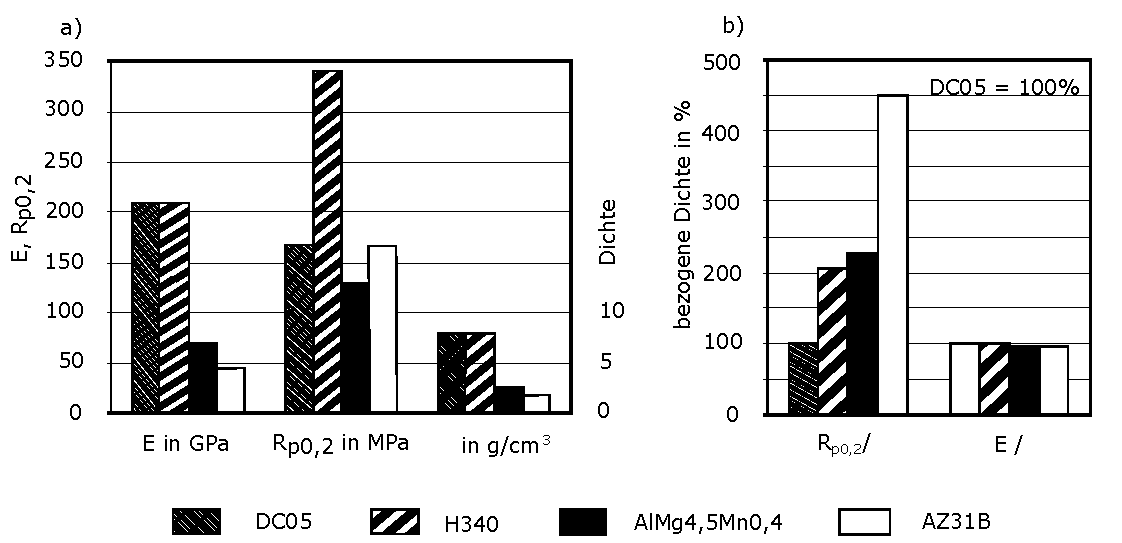
\includegraphics[width=0.9\linewidth]{Bilder/SdT/Eig_Mg}
    \caption[Mechanische Eigenschaften verschiedener Blechwerkstoffe]{Mechanische Eigenschaften verschiedener Blechwerkstoffe nach~\cite{Droeder1999} a) E-Modul, Dehngrenze und Dichte von Stahl, Aluminium und Magnesium, b) spezifisches E-Modul und Dehngrenze}
    \label{fig:Eig_Mg}
\end{figure}

Neben der hohen spezifischen Festigkeit bietet Magnesium ein gutes Dämpfungsvermögen, hohe magnetische Abschirmung und eine gute Wärmeleitfähigkeit~\cite[Aghion.2000].
Dies sind Eigenschaften, die auch im Transportsektor entscheidend für die Anwendung sein können, wie in \autoref{subsec:anwendung} gezeigt wird.
Andere Eigenschaften sind die hohe Beulsteifigkeit von Blechen, hohe elektromagnetische Abschirmung und Wärmeleitfähigkeit sowie die Biokompatibilität~\cite{Brown2015,Aghion2000}.
Daher können Magnesiumwerkstoffe auch in der Elektronikindustrie und Medizintechnik Anwendung finden.

Magnesiumlegierungen können als Guß- oder Knetwerkstoffe verarbeitet und eingesetzt werden.
Mengenmäßig werden Magnesiumwerkstoffe aktuell vor allem in der Gießereitechnik wegen der sehr guten Gusseigenschaften eingesetzt~\cite{AbuFarha2007}.
Knetlegierungen machen nur circa $10\,\%$ der verarbeiteten Magnesiumlegierungen aus~\cite{Lakho2017}.
Diese bieten aufgrund der durch die Umformung induzierte Festigkeitessteigerung und das günstige Umformgefüge vorteilhafte Eigenschaften im Vergleich zum Gußgefüge~\cite{Enss2001}.

\subsection{Umform- und Rekristallisationsverhalten}\label{subsec:umformverhalten}

Magnesium und Magnesiumlegierungen weist eine hexagonal dichtest gepackte Kristallstruktur.
Im Vergleich zu kubischen Strukturen ist die Umformbarkeit bei niedrigen Temperaturen wie Raumtemperatur deutlich geringer.
Um eine gute Umformbarkeit zu gewährleisten, setzt das von-Mises-Kriterium mindestens fünf voneinander unabhängige Gleitsysteme voraus~\cite{Schmidt2011}.

Magnesium bildet bei Raumtemperatur zwei aktive Gleitsysteme (Basalgleiten und Zwillingsbildung), und erfüllt die Bedingung somit nicht.
Der Mechanismus des Basalgleitens in der $(0\,0\,0\,1)$ Basisebene in die dichtest gepackte Richtung $<1\,1\,\bar{2}\,0$ wird in \autoref{fig:basalgleiten} gezeigt.

\begin{figure}[H]%[htbp]
    \centering
    \includegraphics[width=0.6\linewidth]{Bilder/SdT/Basalgleiten}
    \caption[Basalgleitebenen]{Schematische Darstellungen der Basalgleitebenen nach~\cite{Kammer2000}}
    \label{fig:basalgleiten}
\end{figure}

Der Mechanismus der Zwillingsbildung steht für das Umklappen einzelner Kristallgitterbereiche in eine zur Ausgangslage spiegelsymmetrische Zwillingsebene~\cite{Ullmann2014}~.
Dieses Phänomen tritt verstärkt bei niedrigen Temperaturen, großen Körnern und hohen Dehnraten auf~\cite{Ulacia2011,Reh1973}~.
Zwillingssysteme können in Magnesiumlegierungen durch Verkürzung (Druck) oder Dehnung (Zug) der c-Achse der Elementarzelle induziert werden.
Zugzwillingen weisen eine geringere kritische Schubspannung auf und sind leichter zu aktivieren.
Daraus folgt eine Zug-Druck-Anisotropie in den Fließkurvenverläufen von Magnesiumlegierungen, welche in \autoref{fig:z-d-anisotropie} als Fließkurve gezeigt wird.
Durch die unterschiedlichen Dehngrenzen im Druck- und Zugversuch ist die gleichmäßige Umformung der Legierung erschwert.
Daraus folgt eine Asymmetrie der Fließ- und Verfestigungseigenschaften von Magnesiumlegierungen bei der plastischen Formgebung.
Ein herausragendes Beispiel ist die Ausbildung einer ausgeprägten Walztextur beim Walzen von Blechen~\cite{Steglich2014,Schmidt2011}~.

\begin{figure}[H]%[htbp]
    \centering
    \includegraphics[width=0.9\linewidth]{Bilder/SdT/Zug_Druck_Anisotropie}
    \caption[Zug-Druck-Anisotropie]{Darstellung der Zug-Druck-Anisotropie bei AZ31 nach~\cite{Schmidt2011}}
    \label{fig:z-d-anisotropie}
\end{figure}

Die Zwillingsbildung im System $\{1\,0\,\bar{1}\,2\}$ tritt am häufigsten in $<1\,0\,\bar{1}\,1>$ auf.
Dabei kippt die Gitterachse bei einer Zugbelastung der c-Achse um \SI{86}{\degree} um, also annähernd rechtwinklig.
Durch eine Druckbelastung entlang der c-Achse werden Druckzwillinge des $\{1\,0\,\bar{1}\,1\}$ in $<1\,0\,\bar{1}\,2>$ ausgelöst, welche zu einer Verkippung des Gitters um \SI{56}{\degree} führen.
Neben den primären Zwillingsbildungsmechanismen Druck- und Zug-Zwillinge existieren Doppelzwillinge, welche auch als sekundärer Zwillingsmechanismus bezeichnet werden.
Dabei bildet sich ein neuer Zwilling in einem ursprünglichen Zwilling aus.
Es existieren Doppel-Zug-Zwillinge (sekundärer Zugzwilling in primärem Zugzwilling) und auch Doppel-Druck-Zwillinge (sekundärer Druck-Zwilling in primärem Druck-Zwilling)~\cite{Ullmann2014}.

Bei einer Umformung von Magnesiumlegierungen bei Temperaturen von über $\approx$ \SI{225}{\degreeCelsius} steigt das Umformvermögen signifikant an.
Dieser Effekt ist auf die Aktivierung weiterer Gleitsysteme in den Prismenebenen $(1\,\bar{1}\,0\,0)$ entlang der $<1\,1\,\bar{2}\,0>$ Richtung sowie in den Pyramidalebenen erster Ordnung $(1\,\bar{1}\,0\,1)$ in $<1\,1\,\bar{2}\,0>$ Richtung und zweiter Ordnung $(1\,1\,1\,\bar{2}\,2)$ in $<1\,1\,\bar{2}\,\bar{3}>$ Richtung.
In \autoref{fig:pyramidal} werden die Ebenen der Prismengleitung (linker Teil, a) sowie Pyramidalgleitung erster und zweiter Ordnung dargestellt (rechter Teil, b).
Die Temperatur der Aktivierung dieser Gleitsysteme ist vom eingesetzen Legierungssystem abhängig~\cite{Kammer2000}.
Für die Verbesserung des Umformvermögens ist die Aktivierung der Gleitsysteme in den Pyramidalebenen zweiter Ordnung von besonderer Bedeutung~\cite{Enss2001,Doege2010}~.
Sowohl die Basisgleitung, als auch die Prismengleitung und die Pyramidalgleitung erster Ordnung verlaufen entlang der $<1\,1\,\bar{2}\,0>$ Richtung.
Erst mit Aktivierung der Pyramidalgleitung zweiter Ordnung ist eine nicht-basale Versetzungsbewegung entlang der $<1\,1\,\bar{2}\,\bar{3}>$ gegeben und damit das von-Mises-Kriterium vollständig erfüllt~\cite{Schmidt2011}.

\hkl[123] \hkl[-1-2-3]

\begin{figure}[H]%[htbp]
    \centering
    \includegraphics[width=0.9\linewidth]{Bilder/SdT/Gleitsysteme}
    \caption[Gleitsysteme]{Schematische Darstellung der Gleitsysteme a) Prismengleitung | b) Pyramidalgleitung erster und zweiter Ordnung nach~\cite{Kammer2000}}
    \label{fig:pyramidal}
\end{figure}

Um die begrenzte Umformbarkeit der Magnesiumlegierungen bei Raumtemperatur zu erhöhen, ist die Beeinflussung der Korngröße eine angewendete Möglichkeit.
Auch bei niedrigeren Temperaturen kann so durch ein feineres Korn eine deutlich verbesserte Umformbarkeit erreicht werden~\cite{Tripathi2017}.

Die Gründe für dieses Phänomen können wie folgt zusammengefasst werden~\cite{NarayanaMurty2015}:
\begin{enumerate}
    \item Um den Korngrenzenzusammenhalt beizubehalten, werden an den Korngrenzen sowohl basale als auch nicht basale Gleitsysteme aktiviert.
    Bei kleineren Körner reichen diese Korngrenzenzonen bis ins Innere, während sie bei größeren Körnern nur direkt an den Korngrenzen liegen, wodurch im Korninneren vorwiegend ausschließlich basales Gleiten auftritt.
    Im Gegensatz dazu weisen kleinere Körner auch im Inneren beide Arten - basal und nicht-basal - von Gleiten auf.
    \item Für die Rissausbreitung muss die kritische Spannung an den Korngrenzen überschritten sein.
    Diese kritische Spannung ist bei kleinen Körnern höher.
    Somit wird die Rissentwicklung gehemmt und die bis zum Bruch aufnehmbare Dehnung steigt an.
\end{enumerate}

Anhand der ductile to brittle transformation temperature (\s{DBTT}, englisch für Übergangstemperatur vom duktilen zum spröden Zustand) ist der Effekt der kleineren Korngröße auf die Duktilität erkennbar.
Bei einer Korngröße von \SI{60}{\mu m} liegt die Übergangstemperatur von duktilen zu spröden Werkstoffverhalten bei \SI{250}{\degreeCelsius}.
Bei einer Korngröße vo \SI{2}{\mu m} sinkt die DBTT bei Raumtemperatur~\cite{NarayanaMurty2015}.

Bei der Umformung von Magnesium kommt es zur Ausbildung einer Textur oder Vorzugsorientierung aufgrund der hexagonalen Kristallstruktur.
Wirkt während des Umformprozesses eine mechanische Spannung, rotieren die Gleitsysteme in eine bevorzugte Ausrichtung.
Dies geht mit der Richtungsabhängigkeit der mechanischen Eigenschaften einher.
Magnesiumlegierungen weisen nach der Umformung eine sogenannte Basaltextur auf.
Dabei sind die Basalebenen des Kristallgitters parallel zur Blechebene einstellt~\cite{Styczynski2004,Jeong2007}.
\autoref{fig:basaltextur} zeigt im linken Teil eine schematische Darstellung einer ausgeprägten Basaltextur.
Bei dieser Anordnung sind die Grundflächen der Elementarzellen parallel zur Walzrichtung ausgeprägt.
Im rechte Teil ist eine regellose Textur schematisch dargestellt, in der es keine Vorzugsrichtung gibt.
Durch Polfiguren können Texturen dargestellt und verdeutlicht werden.

\begin{figure}[H]%[htbp]
    \centering
    \includegraphics[width=0.9\linewidth]{Bilder/SdT/Basaltextur}
    \caption[Ausgeprägte und nicht ausgeprägte Basaltextur]{a) ausgeprägte Basaltextur | b) nicht ausgeprägte Basaltextur~\cite{Ullmann2019}}
    \label{fig:basaltextur}
\end{figure}

Stutz et al.~\cite{Stutz.2015} untersuchten den Einfluss der Textur auf das Umformverhalten von AZ31 Blechen.
Bei richtungsabhängigen Blechumformprozessen wie beispielsweise Streckziehen zeigt sich der Einfluss der Textur bei unterschiedlichen Temperaturen.
Bei einer stark ausgeprägten Basaltextur kann eine sprunghafte Verbesserung der Umformbarkeit in Dickenrichtung ab einer Temperatur von \SI{200}{\dC} beobachtet werden.
Durch die Aktivierung nicht basaler Gleitsysteme in den Pyramidalebenen zweiter Ordnung können Dickenänderungen deutlich verbessert werden.
Bei erhöhten Temperaturen unter \SI{200}{\dC} verbessern sich zwar die Versetzungsbewegung in prismatischen und basalen Ebenen.
Diese sind parallel zur Blechoberfläche ausgerichtet und tragen nicht zu einer erhöhten Umformbarkeit in Dickenrichtung bei.

Bei einer abgeschwächten Textur ohne gleichmäßig orientierte Körner verbessert sich das Umformvermögen mit steigender Temperatur stetig.
Das kann mit vereinfachten Gleitmechanismen durch andere Gleitsysteme begründet werden, die in entsprechender Kornorientierung auch die Dickenreduzierung ermöglichen~\cite{Stutz2015}.
Eine schwächere Textur kann somit als vorteilhaft für eine bessere Umformbarkeit angesehen werden~\cite{Bettles2005,Yukutake2003}~.
Da Textur in Abhängigkeit der Walz- und Kraftrichtung einstellt, kann durch eine Variation ein weniger intensive Textur erreicht werden~\cite{Chino2007}~.
Die Ausbildung der Textur ist einerseits vom Umformverfahren und Prozessführung abhängig, aber auch von der Legierungszusammensetzung.
Legierungselemente beeinflussen die Aktivierungsenergien von Gleitsystemen und Zwillingsbildung sowie wirkende Rekristallisationsmechanismen, welche die Textur beeinflussen.


\textbf{Rekristallisation} ist eine Entfestigungsprozess bei erhöhter Temperatur, der während (dynamisch) oder nach (statisch) der Umformung ablaufen kann.
Wenn der Entfestigungsprozess während der Umformung beginnt und danach weiterläuft, wird dies als metadynamisch bezeichnet.
Bevor ein Gefüge rekristallisiert, laufen normalerweise Erholungsvorgänge, also die Umordnung und Annihilation von Versetzungen, ab.
Durch den Aufstau von Versetzungen und der darin gespeicherten Energie werden neue Körner durch die Bewegung von Großwinkelkorngrenzen gebildet.
Das neu gebildete Gefüge erweist sich als ärmer an Versetzungen und feiner als das Ausgangsgefüge.
Nach abgeschlossener Rekristallisation kommt es zum Kornwachstum, wobei das Gefüge wieder gröber wird.
Je nach durchlaufenem Rekristallisationsmechanismus gleichen oder unterscheiden sich die Kornorientierungen von altem und neuem Korn~\cite{Ullmann2014}.
Es folgt eine Vorstellung der relevanten Rekristallisationsmechanismen~\cite{Kittner.2019}:

\begin{itemize}
    \item \textbf{Kontinuierliche dynamische Rekristallisation} (continuous dynamic recrystallization = CDRX) zeichnet sich durch eine starke dynamische Erholung aus.
    Versetzungen stauen sich an den Korngrenzen und Zwillingen auf und Erhöhen die lokale Versetzungsdichte.
    Durch Umordnung entstehen erst Kleinwinkelkorngrenzen (KWKG), bei weiteren Versetzungen wandeln sich diese in Großwinkelkorngrenzen (GWKG).
    CDRX tritt bei Temperaturen von über \SI{300}{\degreeCelsius} auf und führt zur gleichgerichteten Orientierung von rekristallisiertem und nicht rekristallisiertem Korn~\cite{NarayanaMurty.2015}.
    \item \textbf{Partikelinduzierte Rekristallisation} (particle stimulated recrystallization = PSN) setzt Ausscheidungen und andere Partikel als Keimstellen voraus.
    Kleine und feindispers verteilte Ausscheidungen (<\SI{1}{\mum}) führen zu einer verlangsamten Rekristallisation.
    Größere Partikel mit einem Durchmesser von über \SI{1}{\mum} beschleunigen den Prozess~\cite{Kittner.2019}.
    Das neu gebildete Gefüge hat keine ausgerichtete Textur, da die Kristallorientierung von der Lage der Partikel abhängt~\cite{Ullmann2019}.
    Der Anteil an der Texturentwicklung ist gering, da im Vergleich zu CDRX deutlich weniger Gefüge in PSN rekristallisiert~\cite{Ullmann2014}.
    \item \textbf{Zwillingsinduzierte Rekristallisation} (twinning-aided dynamic recrystallization = TDRX) basiert auf Zwillingsbildung im Gefüge.
    Die Zwillingskorngrenzen weisen eine erhöhte Gitterverzerrung auf und fungieren als Keimstellen für die dynamische Rekristallisation.
    TDRX beginnt mit der Keimbildung, darauf folgt die Umwandlung von KWKG in reguläre Korngrenzen, welche daraufhin doe Position ändern.
    TDRX findet vorrangig an Druckzwillingen statt, da diese eine höhere Versetzungsdichte als Zugzwillinge aufweisen.
    Da bei der Gefügeneubildung die Kornorientierung rotiert wird, können somit bei der Umformung auch mehr Gleitsysteme die Umformung in Dickenrichtung unterstützen.
    Im letzten Schritt wandeln sich Korngrenzen zu GWKG um~\cite{Kittner.2019}.
\end{itemize}

Sowohl die auftretenden Rekristallisationsmechanismen, als auch mechanische und physikalische Eigenschaften variieren mit den eingesetzen Legierungselementen und -systemen.
Durch den gezielten Einsatz bestimmter Legierungselemente können einzelne Rekristallisationsmechanismen wie TDRX oder PSN verstärkt werden.
So kann eine Randomisierung der Textur erreicht werden und damit Festigkeit und Umformbarkeit verbessert werden.

Zu den klassischen Legierungselementen für Magnesiumlegierungen zählen unter anderem Aluminium, Zink, Silicium und Mangan.
Weiterhin werden teilweise Seltene Erden und Calcium eingesetzt, um die Eigenschaften zu modifizieren~\cite{Rout2020}.
Calcium (Element Ca, in Magnesiumlegierungen als X) erhöht die Kriechbeständigkeit und Festigkeit durch Ausscheidungsbildung.
Durch eine Abschwächung der Textur wird eine verbesserte Umformbarkeit erreicht.
Weitere Eigenschaften sind geringere Entflammbarkeit und eine verbesserte Hochtemperaturfestigkeit~\cite{Yi2016}.

Die bisher am umfangreichsten eingesetzte Magnesiumknetlegierung ist die Legierung AZ31 (\SI{3}{\percent} Al, \SI{1}{\percent} Zn, Angabe in Masse-\SI{}{\percent}).
Der Werkstoff weist durch das verwendete Legierungssystem eine hohe spezifische Festigkeit auf~\cite{Droeder1999}.
Aufgrund einer ausgeprägten Basaltextur weisen Werkstücke dieser Legierung geringe Dehnungswerte auf, verglichen mit anderen Legierungssysteme~\cite{Stutz2015}.


\subsection{Magnesiumlegierung ZAX210}\label{subsec:zax}

Die Magnesiumlegierung ZAX210 ($\approx$ \SI{2,3}{\percent} Zn, \SI{0,9}{\percent} Al, <\SI{0,25}{\percent} Ca in Masse-\SI{}{\percent}) weist hinsichtlich der Texturentwicklung eine ungleichmäßige Kristallausrichtung auf.
Im Vergleich mit der Legierung ZE10 (enthält seltene Erden) weist ZAX210 einen stärkeren sogenannten Basalpolsplit auf, also die Streuung der Basaltextur.
Im Vergleich zu AZ31 weisen ZE10 und ZAX210 geringe Werte hinsichtlich der Zugfestigkeit und Streckgrenze auf.
Die Dehnungswerte von ZAX210 sind gleichmäßiger und teils deutlich höher als die von AZ31~\cite{Ullmann2019}.

Mehrere Untersuchungen zeigten die gute Umformbarkeit von ZAX210 bei Raumtemperatur und bei erhöhten Temperaturen~\cite{Ullmann2019,Laser2008}


\begin{table}
    \centering
    \begin{tabular}{| l | l | l | l | l | l | l |}
        %\toprule
        %\multirow{2}*{\textbf{Legierung}} & \multicolumn{3}*{\textbf{Zugfestigkeit in \SI{}{\MPa}}} & & & \multicolumn{3}*{\textbf{Bruchdehnung}} &  &  &  \\
        %\midrule
        % & \textbf{WR} & \textbf{\SI{45}{\degree} zu WR} & \textbf{\SI{90}{\degree} zu WR} & \textbf{WR} & \textbf{\SI{45}{\degree} zu WR} & \textbf{\SI{90}{\degree} zu WR} \\
        \hline
        Legierung & \textbf{Zugfestigkeit in \SI{}{\MPa}} & & & \textbf{Bruchdehnung} & & \\
        \hline
        AZ31 & 277 & 275 & 271 & 26 & 18 & 14 \\
        \hline
        ZAX210 & 243 & 234 & 236 & 30 & 32 & 26 \\
        \hline
        % \bottomrule
    \end{tabular}
    \caption{mechanische Eigenschaften gießgewalzter und gewalzter Bleche nach der Abschlusswärmebehandlung nach~\cite{Ullmann2019}}
    \label{tab:}
\end{table}


\subsection{Eigenschaften und Herstellung von Magnesium-Gießband}\label{subsec:eigherstellungmgband}

\subsection{Oberflächenvorbehandlungen und Einflüsse}\label{subsec:oberflächen}

%\nomtypeL[F]{$F$}{Kraft}{N}
%\nomtypeL[Fi]{$F_i$}{innere Kraft}{N}
%\nomtypeL[tg]{$T_g$}{Glasübergangstemperatur}{$^\circ\text{C}$}
%\nomtypeL[Aw]{$A_w$}{wahre Oberfläche}{$mm^2$}
%\nomtypeL[rpm]{rpm}{rounds per minute, Umdrehungen pro Minute}{$s^{-1}$}

%%\nomtypeG[varphi]{$\varphi$}{Umformgrad}{[-]}
%\nomtypeG[sigmaH]{$\sigma _H$}{Haftung}{\frac{N}{mm}}

%\nomtypeA[FML]{FML}{Fibre Metal Laminate}
%\nomtypeA[AW]{AW}{Aluminiumwerkstoff}
%\nomtypeA[Glare]{Glare}{Glass Reinforced Aluminium Laminate}
%\nomtypeA[Arall]{Arall}{Aramid Reinforced Aluminium Laminate}
%\nomtypeA[Carall]{Carall}{Carbon Fibre Reinforced Aluminium Laminate}
%\nomtypeA[Mg]{Mg}{Magnesium}
%\nomtypeA[Zn]{Zn}{Zink}
%\nomtypeA[Al]{Al}{Aluminium}
%\nomtypeA[Ni]{Ni}{Nickel}
%\nomtypeA[PA]{PA}{Polyamid}
%\nomtypeA[PP]{PP}{Polypropylen}
%\nomtypeA[PP]{PP}{Polypropylen}\nomtypeA[PP]{PP}{Polypropylen}